In this chapter, we will delve into the implementation and validation of our testing procedures for the Oracle Linux Virtualization and System Testing project. We will begin by outlining the technical choices and configurations used in our tests. Subsequently, we will describe each test in detail, including the setup, execution, and analysis of results.

\newpage
\fancyhead[R]{\textsc{Chapter 4 - Tests Realization and Results}}
\hypertarget{fourthchapter}{}

%% Manual QEMU 7.2.0-14 OCI Intel Host OL8+UEK7U2 Guest: OL 8.9 + UEK7U2
\section{Test on OL8 Host with an Intel CPU, QEMU and latest kernel version UEK7U2}

%% Information about Host
\subsection{Host System Configuration}

To begin the testing process, we set up an Intel-based host running Oracle Linux Server 8.10, which utilizes the x86-64 architecture. The system was further configured with the latest version of the UEK7U2. To verify the environment, the hostnamectl command was executed, confirming the successful installation and configuration:

\begin{center}
    \centering
    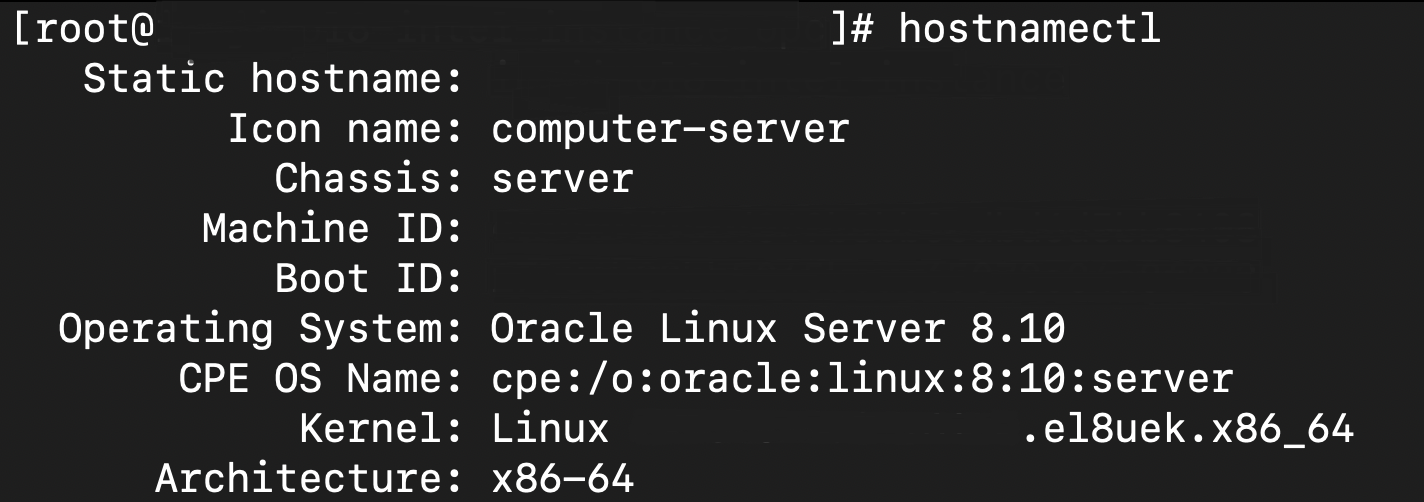
\includegraphics[width=\textwidth]{Images/Hostnamectl Command on the Host.png}
    \captionof{figure}{Verification of Host Configuration Using hostnamectl Command}
    \label{fig:casa}
\end{center}

After the host environment was confirmed, QEMU was installed. The successful installation of QEMU and its associated packages was verified using the yum command, which displayed all the installed components, including qemu-img, qemu-kvm, and several QEMU-related modules:

\begin{center}
    \centering
    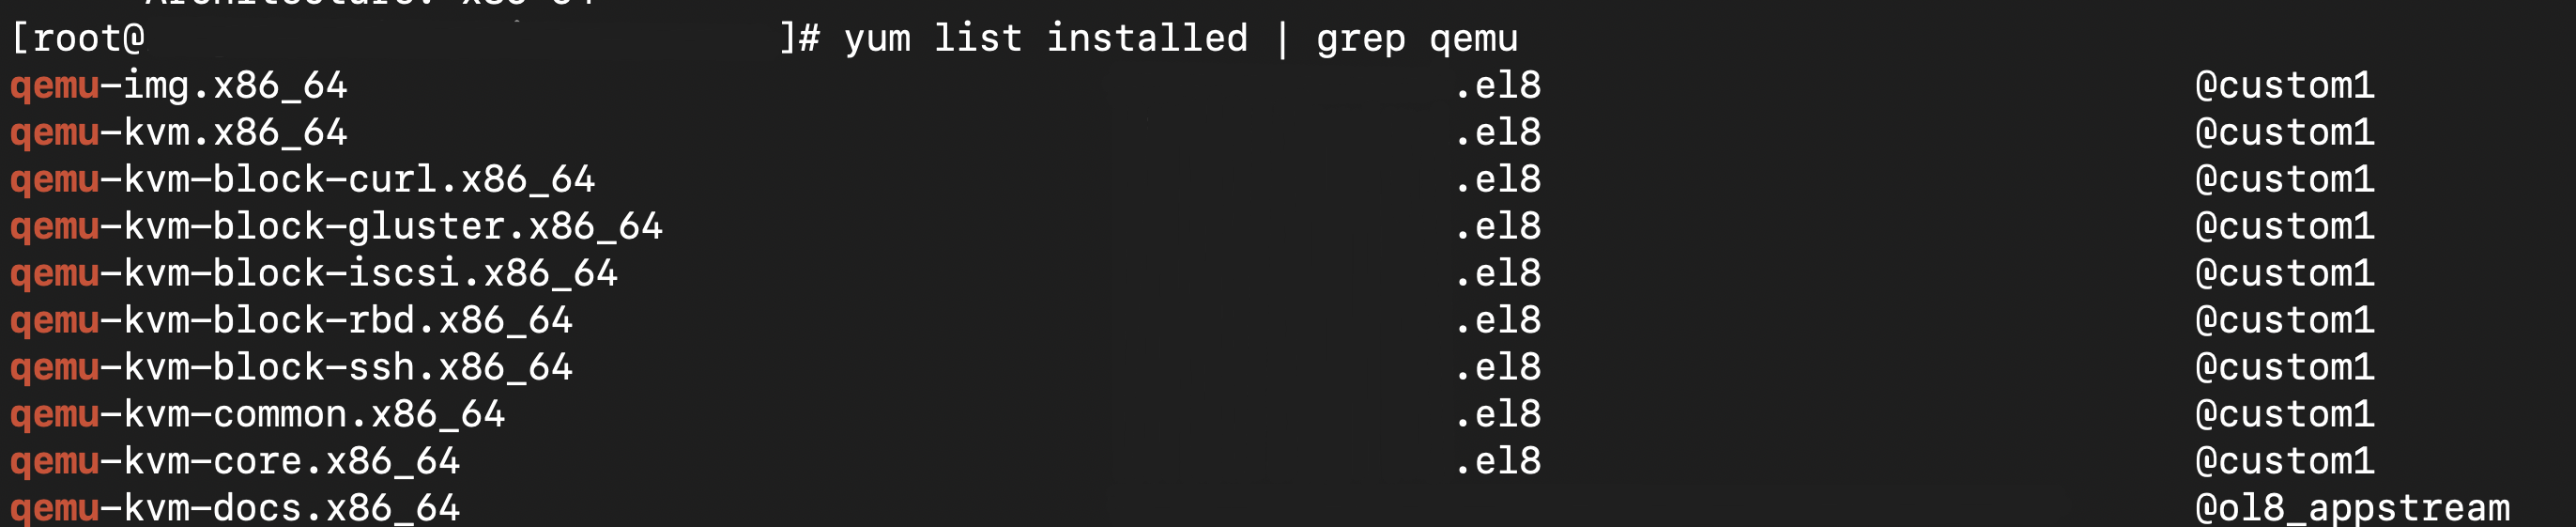
\includegraphics[width=\textwidth]{Images/QEMU Version_ 7.2.0-14 oci.png}
    \captionof{figure}{Installed QEMU Version Verification}
    \label{fig:casa}
\end{center}

Furthermore, we confirmed the presence of OVMF files and checked the edk2 package to ensure that the necessary UEFI components were available. These files are critical for running UEFI-based virtual machines:

\begin{center}
    \centering
    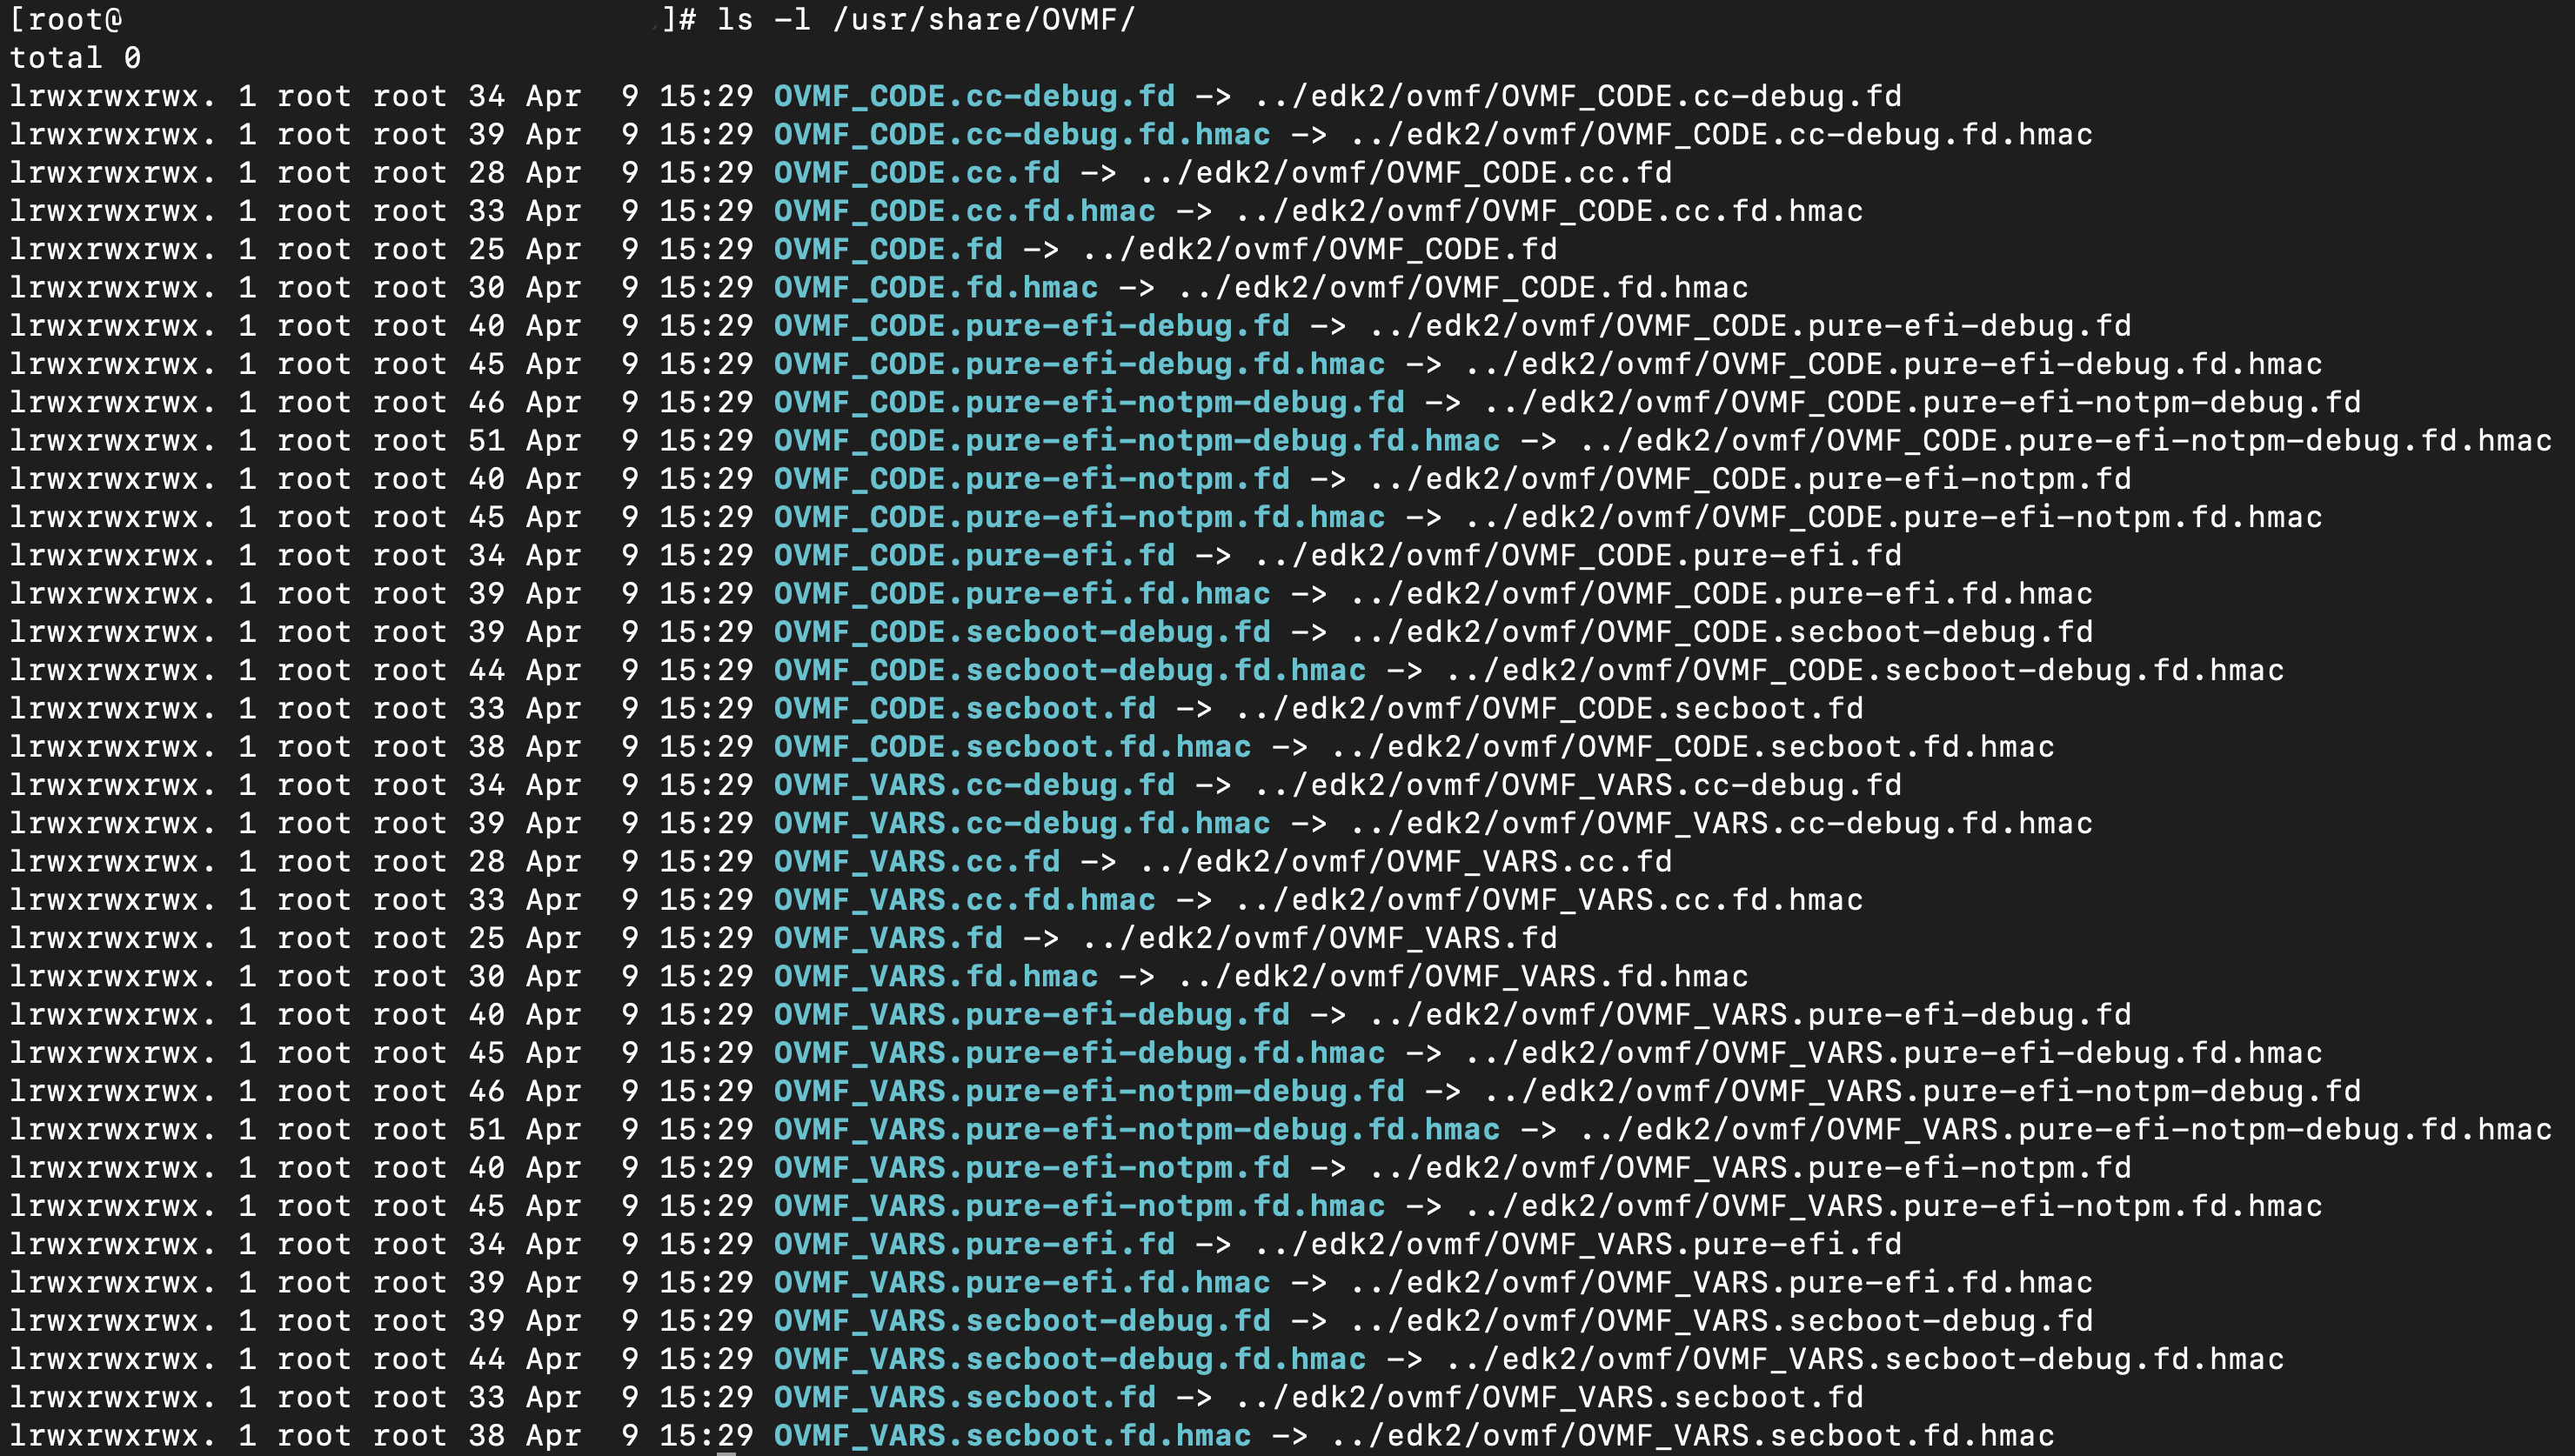
\includegraphics[width=\textwidth]{Images/OVMF Folder.png}
    \captionof{figure}{Checking UEFI Components in OVMF Directory}
    \label{fig:casa}
\end{center}

\begin{center}
    \centering
    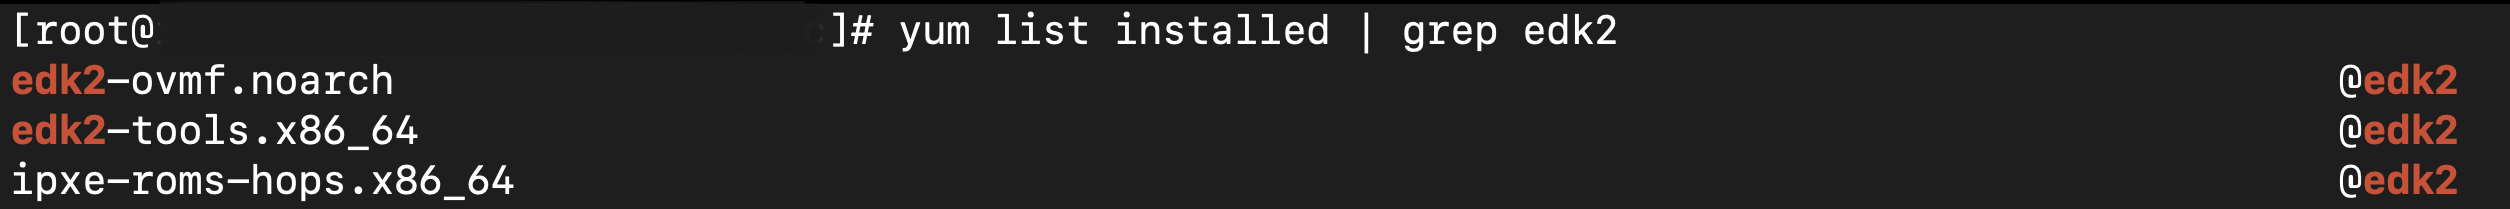
\includegraphics[width=\textwidth]{Images/edk2 Version.png}
    \captionof{figure}{Verifying edk2 Version for UEFI Compatibility}
    \label{fig:casa}
\end{center}

To ensure the system had sufficient resources for running and testing virtual machines, we recorded the available storage and memory using the df -h and lsmem commands, respectively. This information is crucial for the development team to troubleshoot any issues related to resource allocation during the testing process:

\begin{center}
    \centering
    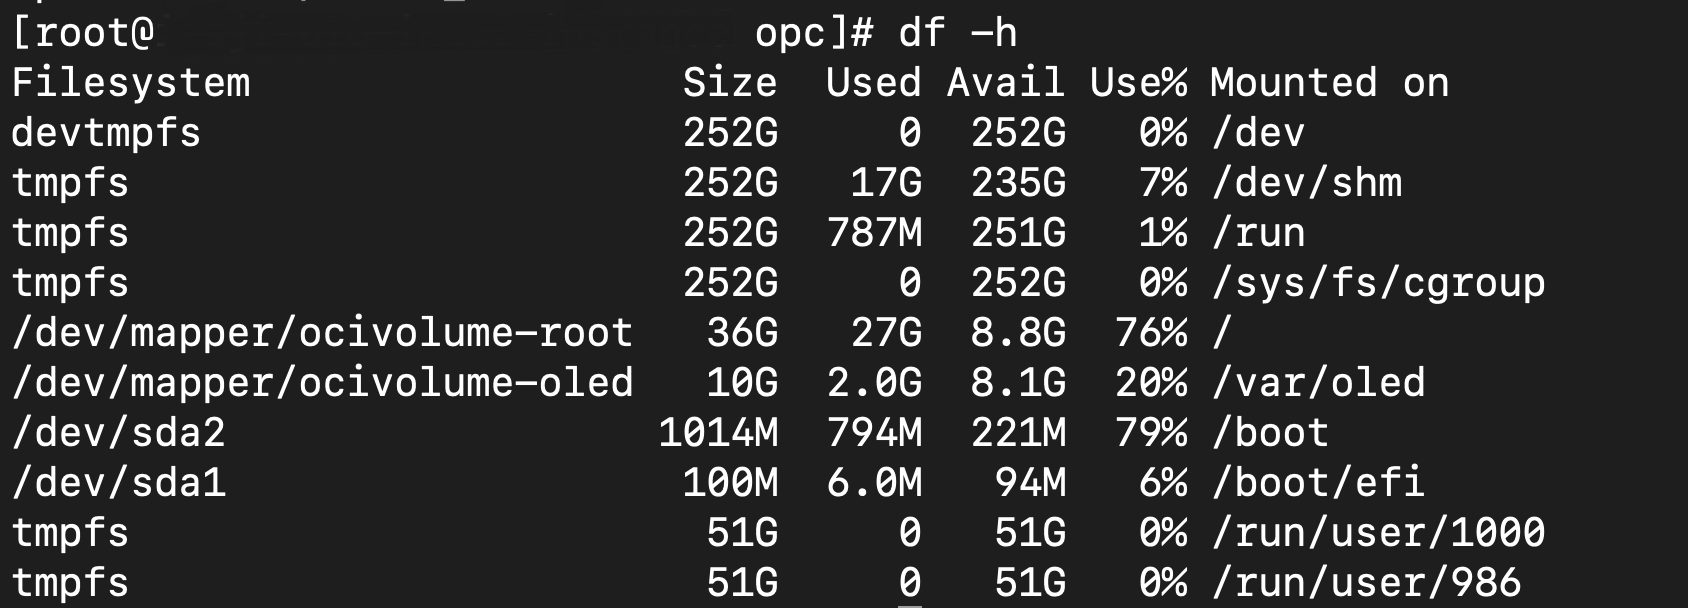
\includegraphics[width=\textwidth]{Images/Storage on the Host.png}
    \captionof{figure}{Available Storage Capacity on Host System}
    \label{fig:casa}
\end{center}

\begin{center}
    \centering
    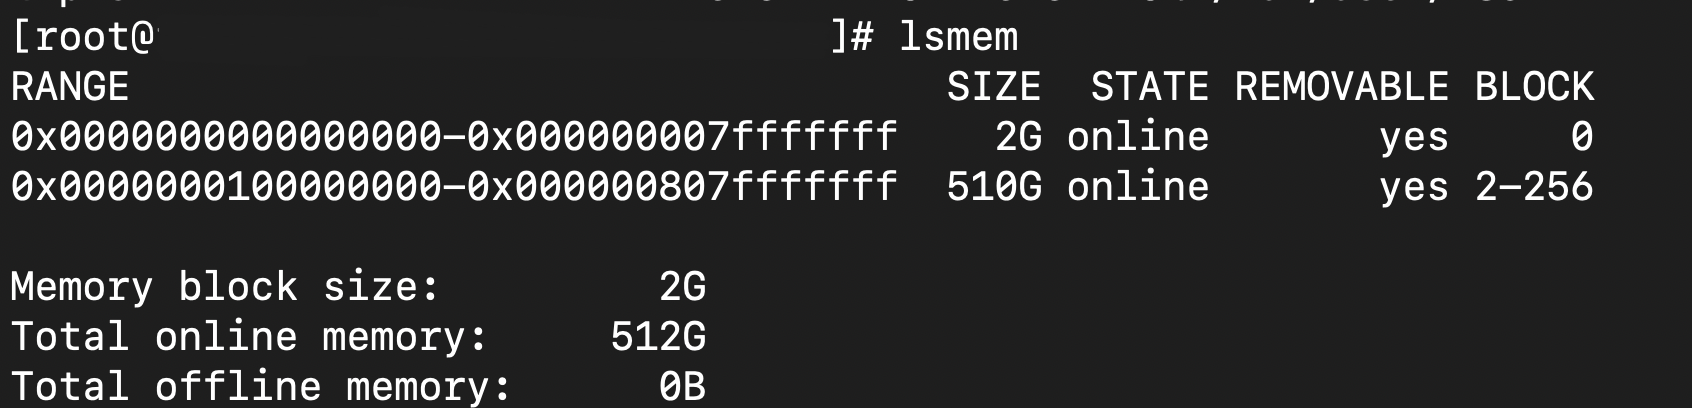
\includegraphics[width=\textwidth]{Images/Memory on the Host.png}
    \captionof{figure}{Host Memory Information}
    \label{fig:casa}
\end{center}

%% Running the Guest
\subsection{Guest Virtual Machine Deployment}
With the host system fully configured, we proceeded to run the guest VM. The VM was initiated using the following QEMU command, which defined various parameters including memory allocation, CPU cores, and disk images. This command ensured that the VM was properly configured to mirror a typical production environment:

\begin{center}
    \centering
    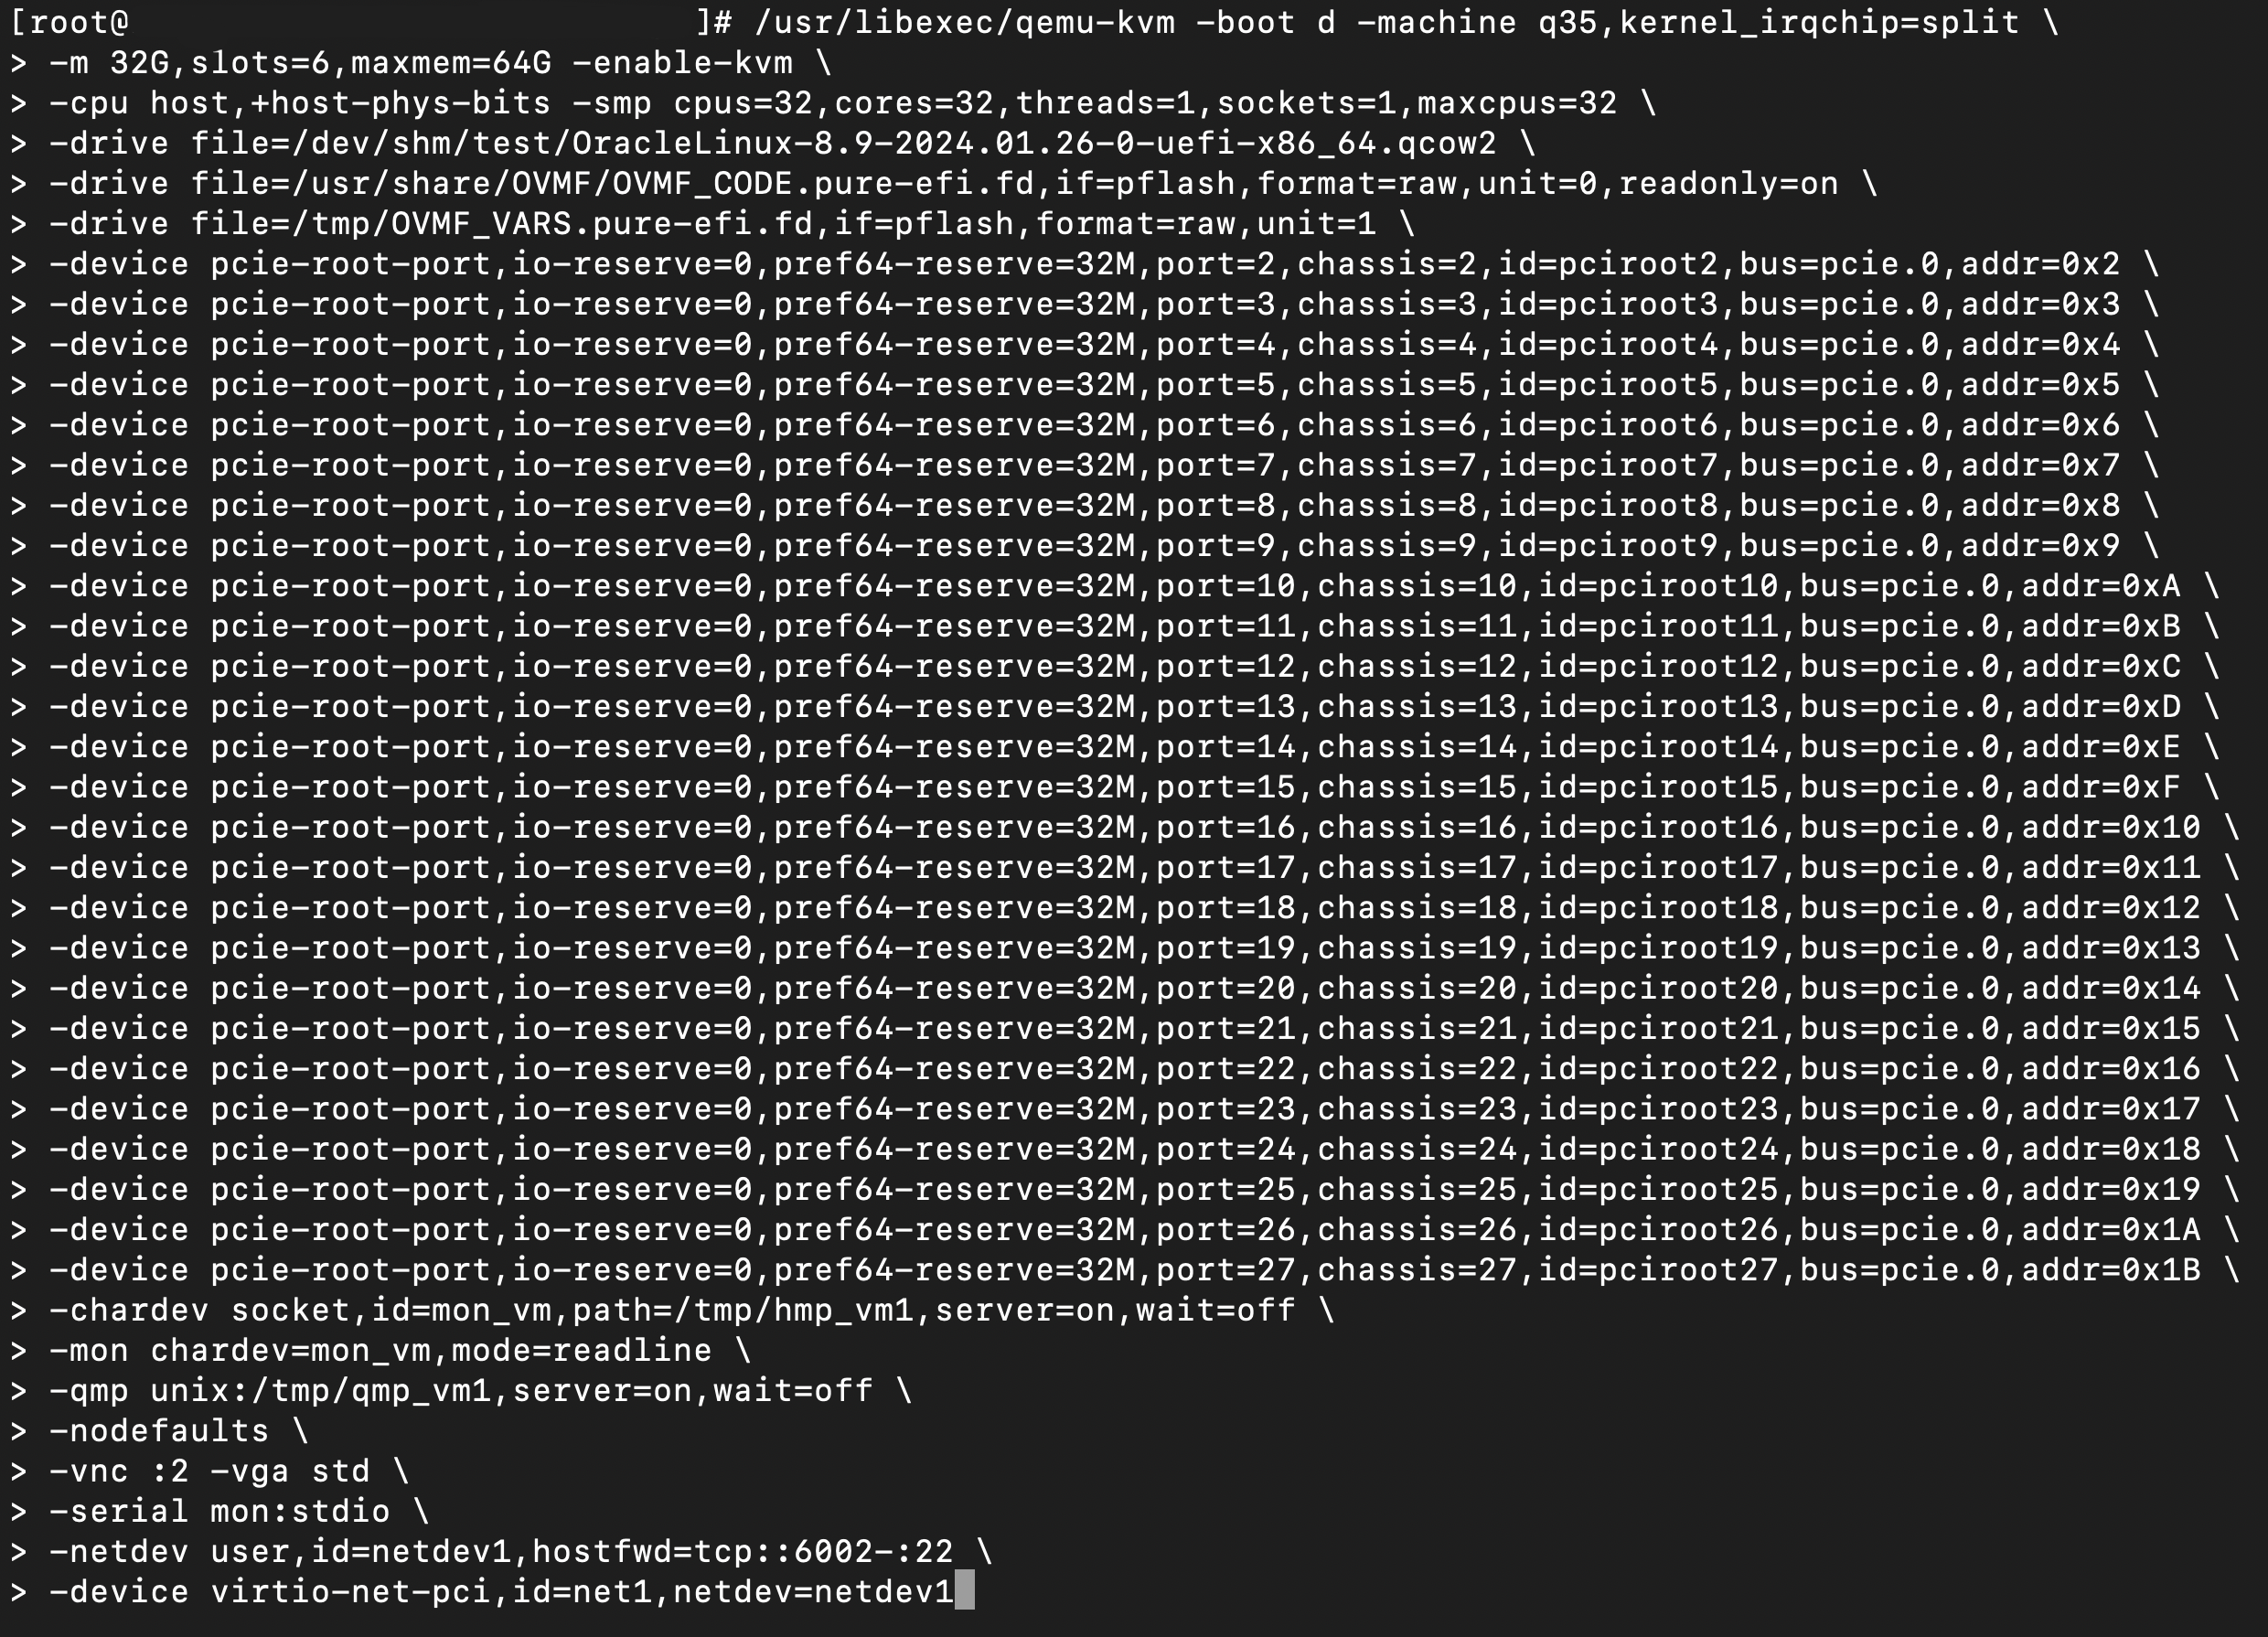
\includegraphics[width=\textwidth]{Images/Launching the Guest.png}
    \captionof{figure}{Launching Guest VM with QEMU Command}
    \label{fig:casa}
\end{center}

After launching the guest, we confirmed that it was running Oracle Linux Server 8.9 with UEK7U2. This was verified by executing the hostnamectl and uname -r commands within the guest VM:

\begin{center}
    \centering
    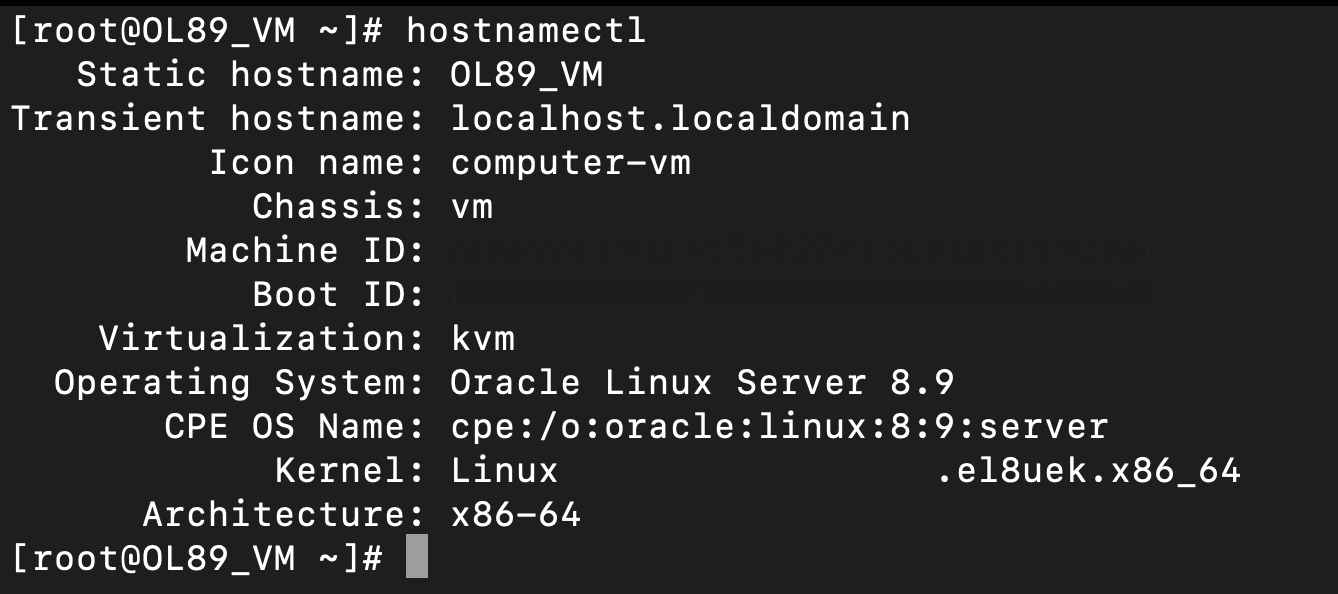
\includegraphics[width=\textwidth]{Images/Hostnamectl Command on the Guest.png}
    \captionof{figure}{Verifying Hostname within the Guest}
    \label{fig:casa}
\end{center}

\begin{center}
    \centering
    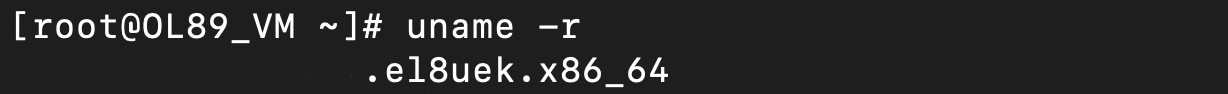
\includegraphics[width=\textwidth]{Images/Uname -r Command on the Guest.png}
    \captionof{figure}{Kernel Version Verification in Guest}
    \label{fig:casa}
\end{center}

This verification confirmed that the VM was correctly set up and ready for the subsequent testing procedures.


%% Tests
\subsection{Test Execution and Performance Evaluation}
To evaluate the stability and performance of the virtual environment, a series of tests were conducted. These tests focused on the VM's lifecycle operations, networking capabilities, and its ability to handle hotplug and unplug events for multiple virtual network interfaces.

%% Lifecycle Test
\subsubsection[Lifecycle Test]{Lifecycle Test}
The lifecycle test aimed to verify the VM's ability to handle common operational states, such as rebooting, stopping and continuing operations, suspending and waking, and shutting down. Each of these states was carefully tested to ensure that the VM could transition smoothly without any issues.

\begin{itemize}
    \item \textbf{Reboot Test: }\\
          The VM was subjected to a reboot operation using the system\_reset command from the QEMU monitor. This command initiated a full system reboot, simulating scenarios where the VM might need to restart due to system updates or other maintenance tasks. Upon issuing the command, the VM successfully rebooted, with all services coming back online without errors. The logs were checked to confirm that no anomalies occurred during the reboot process.
          \begin{center}
              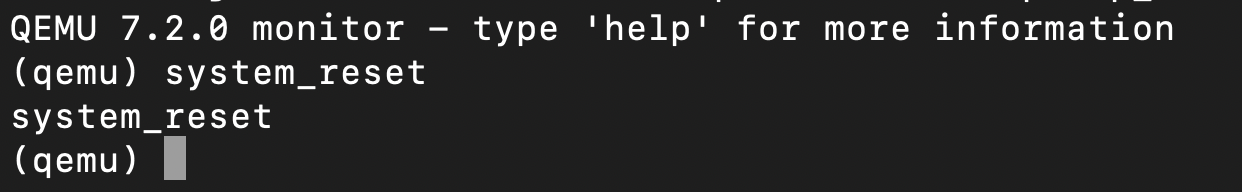
\includegraphics[width=\linewidth]{Images/Rebooting the Guest.png}
              \captionof{figure}{Execution of Reboot Command}
              \label{fig:reboot}
          \end{center}

          After reboot, the guest was checked for uptime and kernel version to ensure that it was the same system with no inconsistencies:
          \begin{center}
              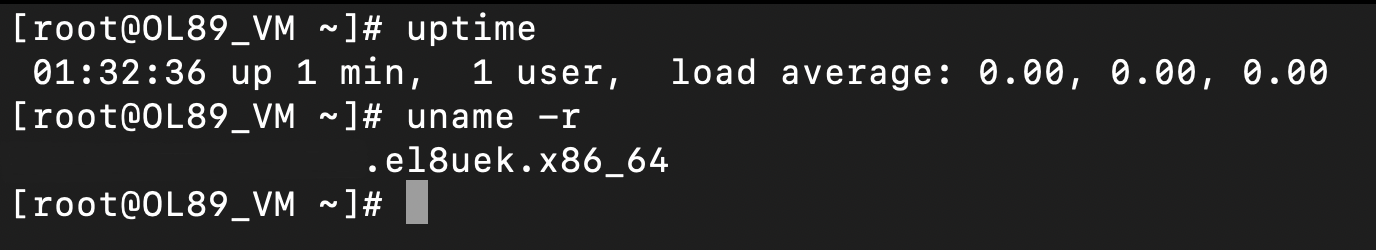
\includegraphics[width=\linewidth]{Images/After Rebooting on the Guest.png}
              \captionof{figure}{Post-Reboot Guest Verification}
              \label{fig:areboot}
          \end{center}

    \item \textbf{Stop/Continue Test:}\\
          In this test, the VM was temporarily stopped using the stop command in the QEMU monitor. This action simulates a scenario where the VM might be paused during a maintenance window or to free up resources temporarily. The VM was then resumed using the cont command. Throughout this process, the VM's state was preserved, and it resumed operations seamlessly.
          \begin{center}
              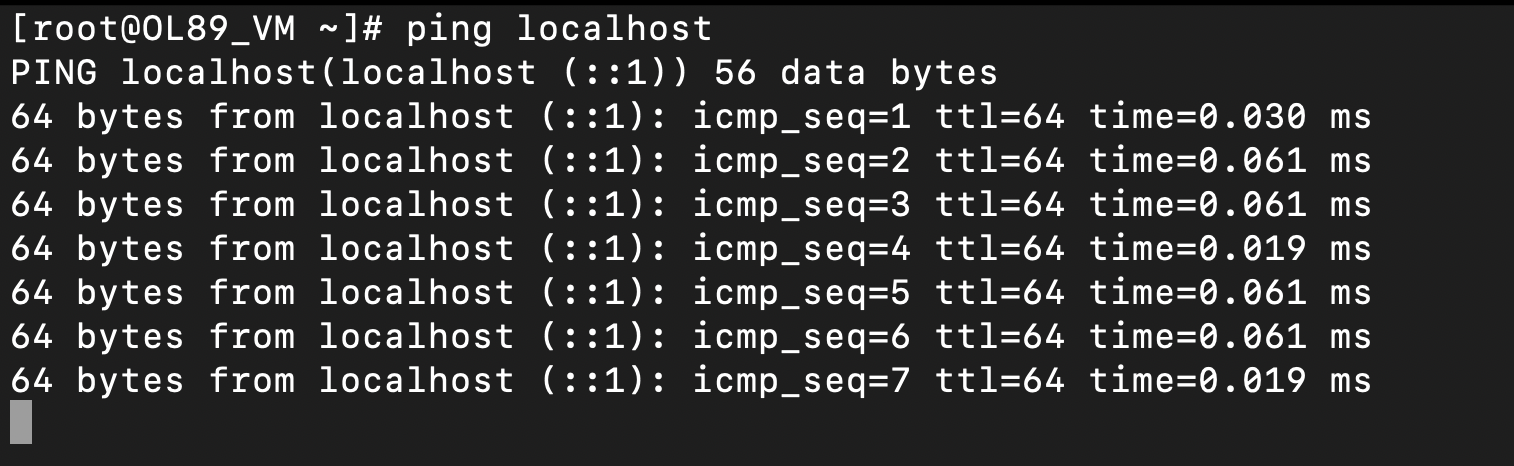
\includegraphics[width=\linewidth]{Images/Ping Localhost When Stop.png}
              \captionof{figure}{Network Connectivity During VM Stop Operation}
              \label{fig:areboot}
          \end{center}
          \begin{center}
              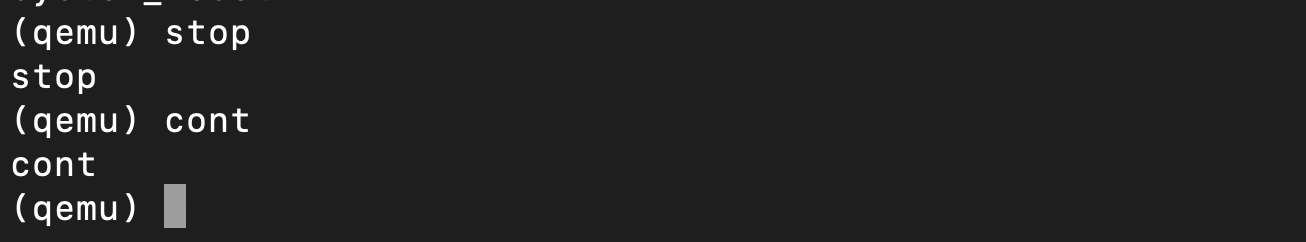
\includegraphics[width=\linewidth]{Images/Stop-Cont Commands.png}
              \captionof{figure}{Stop/Cont Commands Executed on the Guest}
              \label{fig:areboot}
          \end{center}
          \begin{center}
              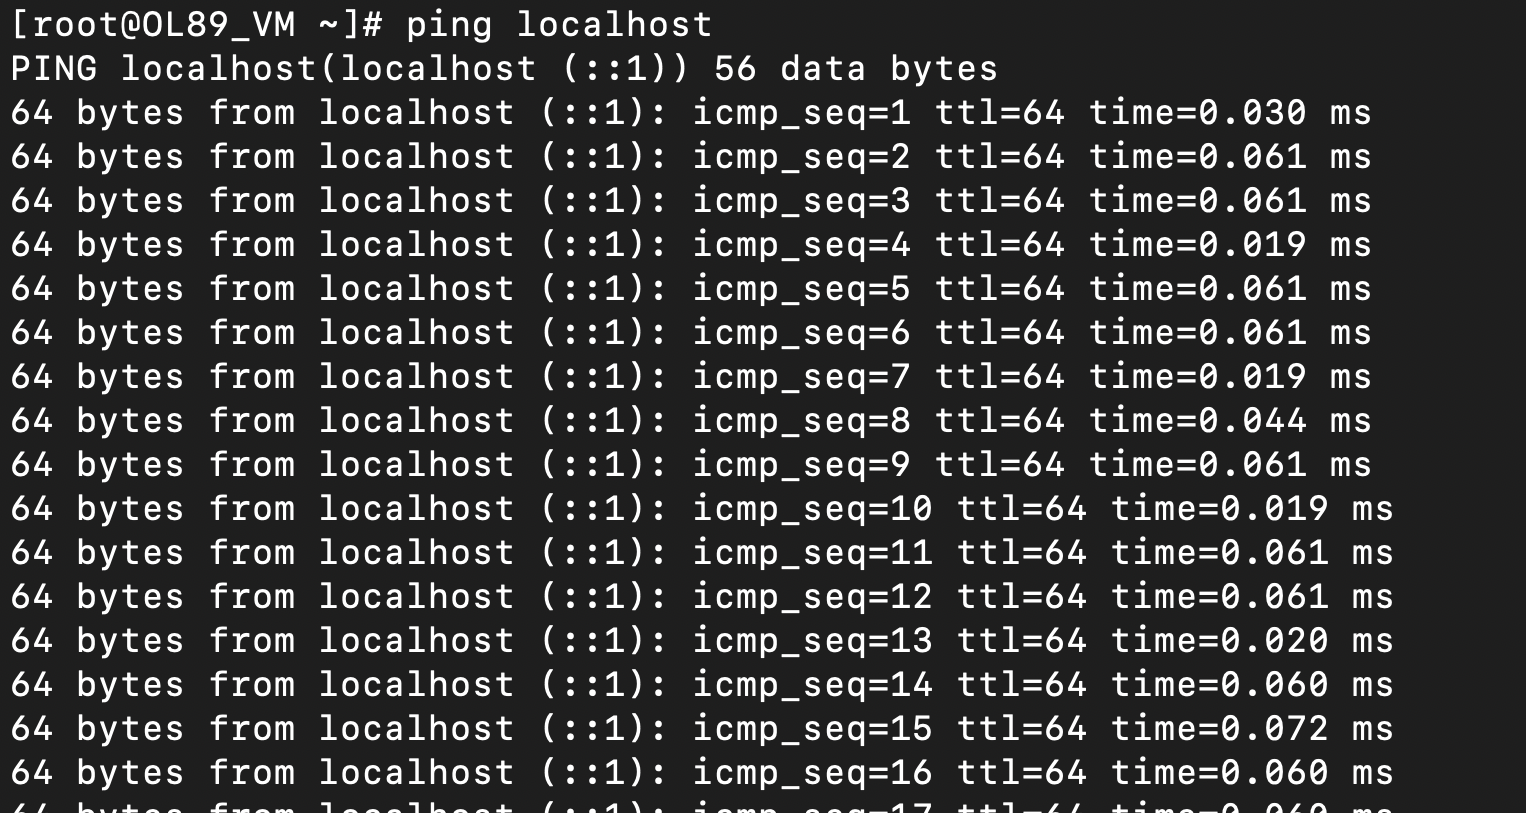
\includegraphics[width=\linewidth]{Images/Ping Localhost After Cont.png}
              \captionof{figure}{Network Connectivity After Resuming VM}
              \label{fig:areboot}
          \end{center}
          Upon continuation, network connectivity, application services, and system responsiveness were all confirmed to be intact.

    \item \textbf{Suspend Test:}\\
          The suspend operation was tested to simulate putting the VM into a low-power state. The systemctl suspend command was used within the guest to initiate this state. The wakeup was triggered using the system\_wakeup command from the QEMU monitor, bringing the VM back to an active state.
          \begin{center}
              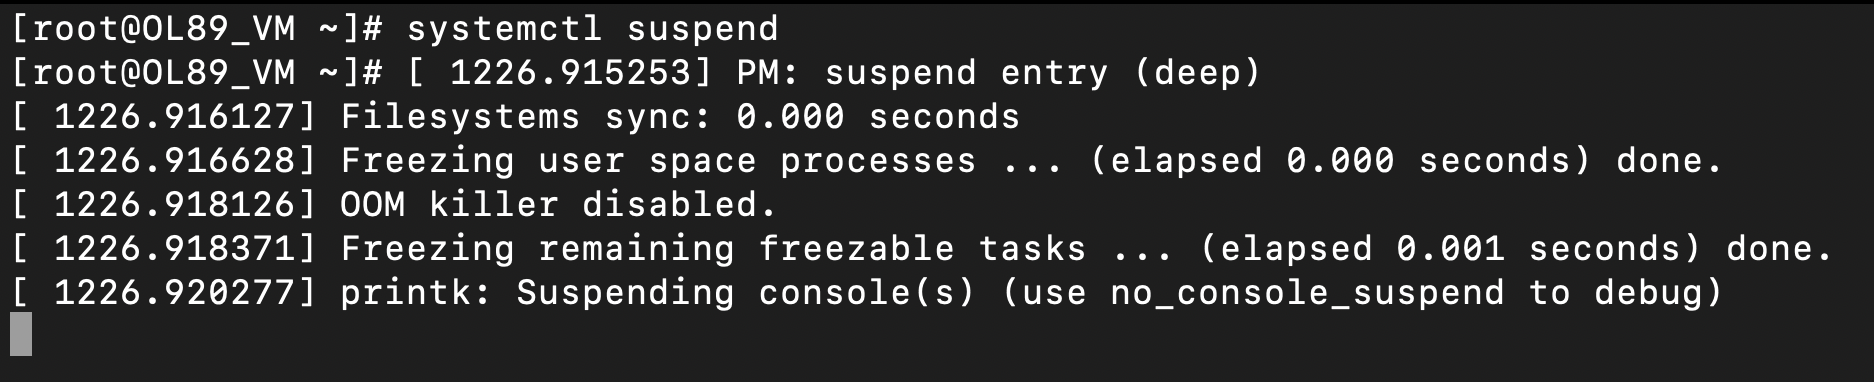
\includegraphics[width=\linewidth]{Images/Systemctl Suspend on the Guest.png}
              \captionof{figure}{Guest VM Suspension Executed}
              \label{fig:areboot}
          \end{center}
          \begin{center}
              \includegraphics[width=\linewidth]{Images/System\_Wakeup.png}
              \captionof{figure}{Executing Wakeup Command via QEMU Monitor}
              \label{fig:areboot}
          \end{center}
          \begin{center}
              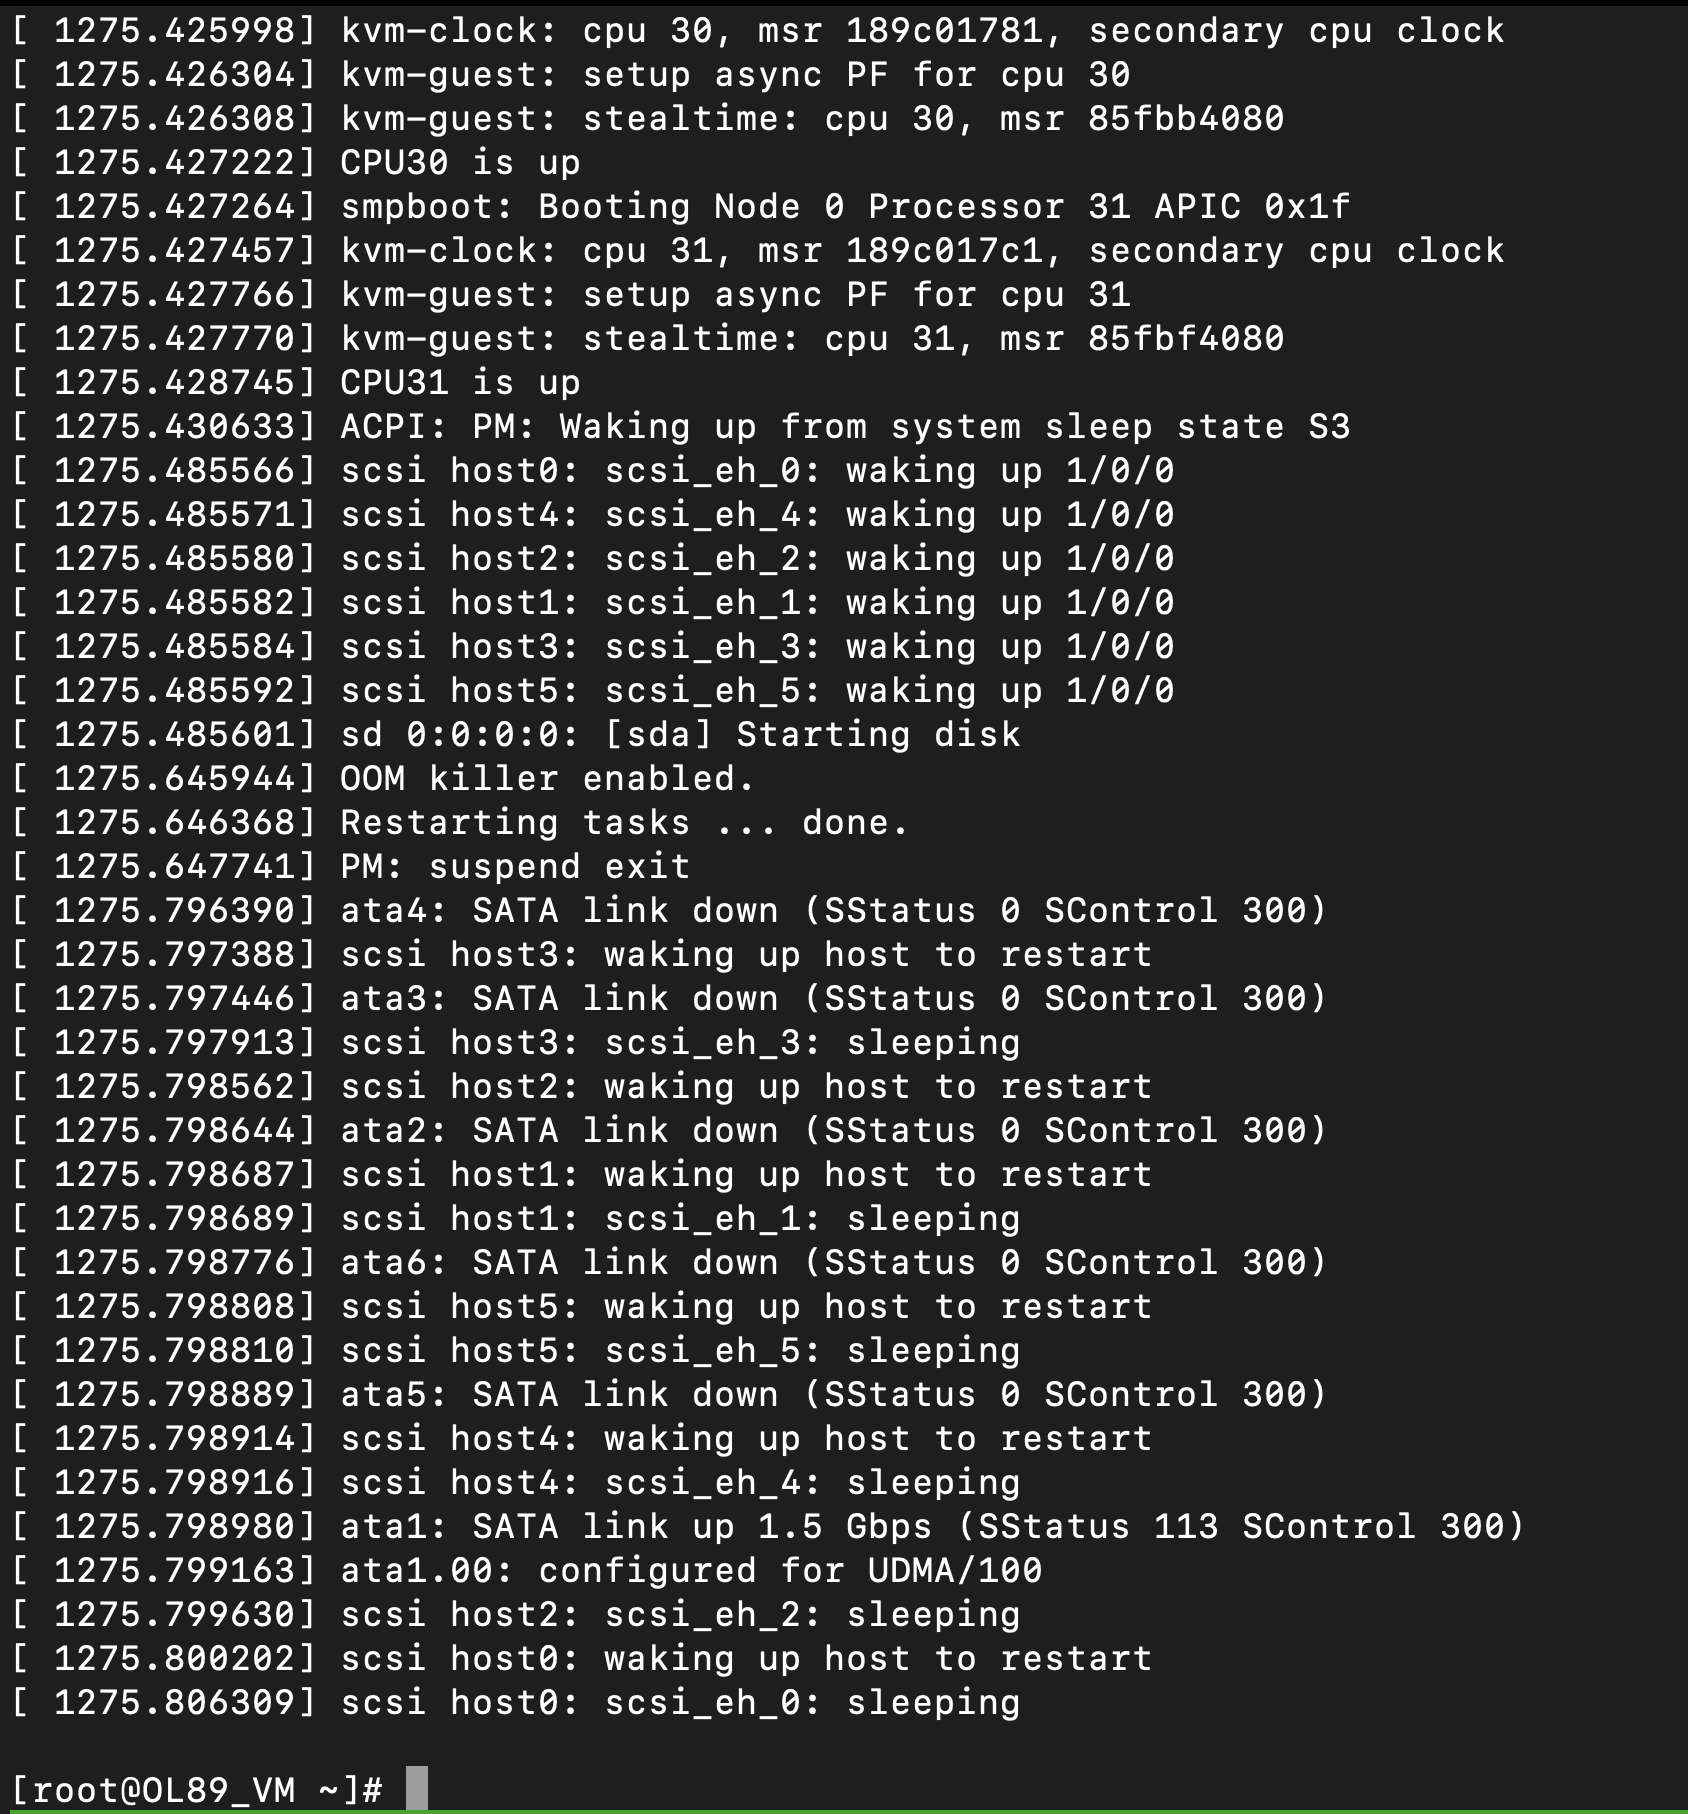
\includegraphics[width=\linewidth]{Images/Wakeup Guest after Suspending.png}
              \captionof{figure}{Verifying the Guest After Wakeup}
              \label{fig:areboot}
          \end{center}
          The VM successfully transitioned in and out of the suspend state, with all previously running processes and services continuing from where they left off. Network connectivity was reestablished without any manual intervention.

    \item \textbf{Shutdown Test:}\\
          Finally, the VM was cleanly shut down using the system\_powerdown command in the QEMU monitor. This test is crucial as it ensures that the VM can safely terminate its operations and power down without data loss or corruption.
          \mynewline
          \mynewline
          \begin{center}
              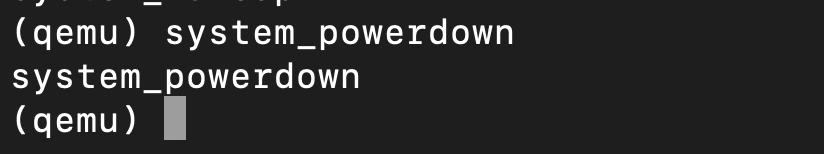
\includegraphics[width=\linewidth]{Images/System-powerdown.png}
              \captionof{figure}{Executing Shutdown Test on the Guest}
              \label{fig:a}
          \end{center}
          \begin{center}
              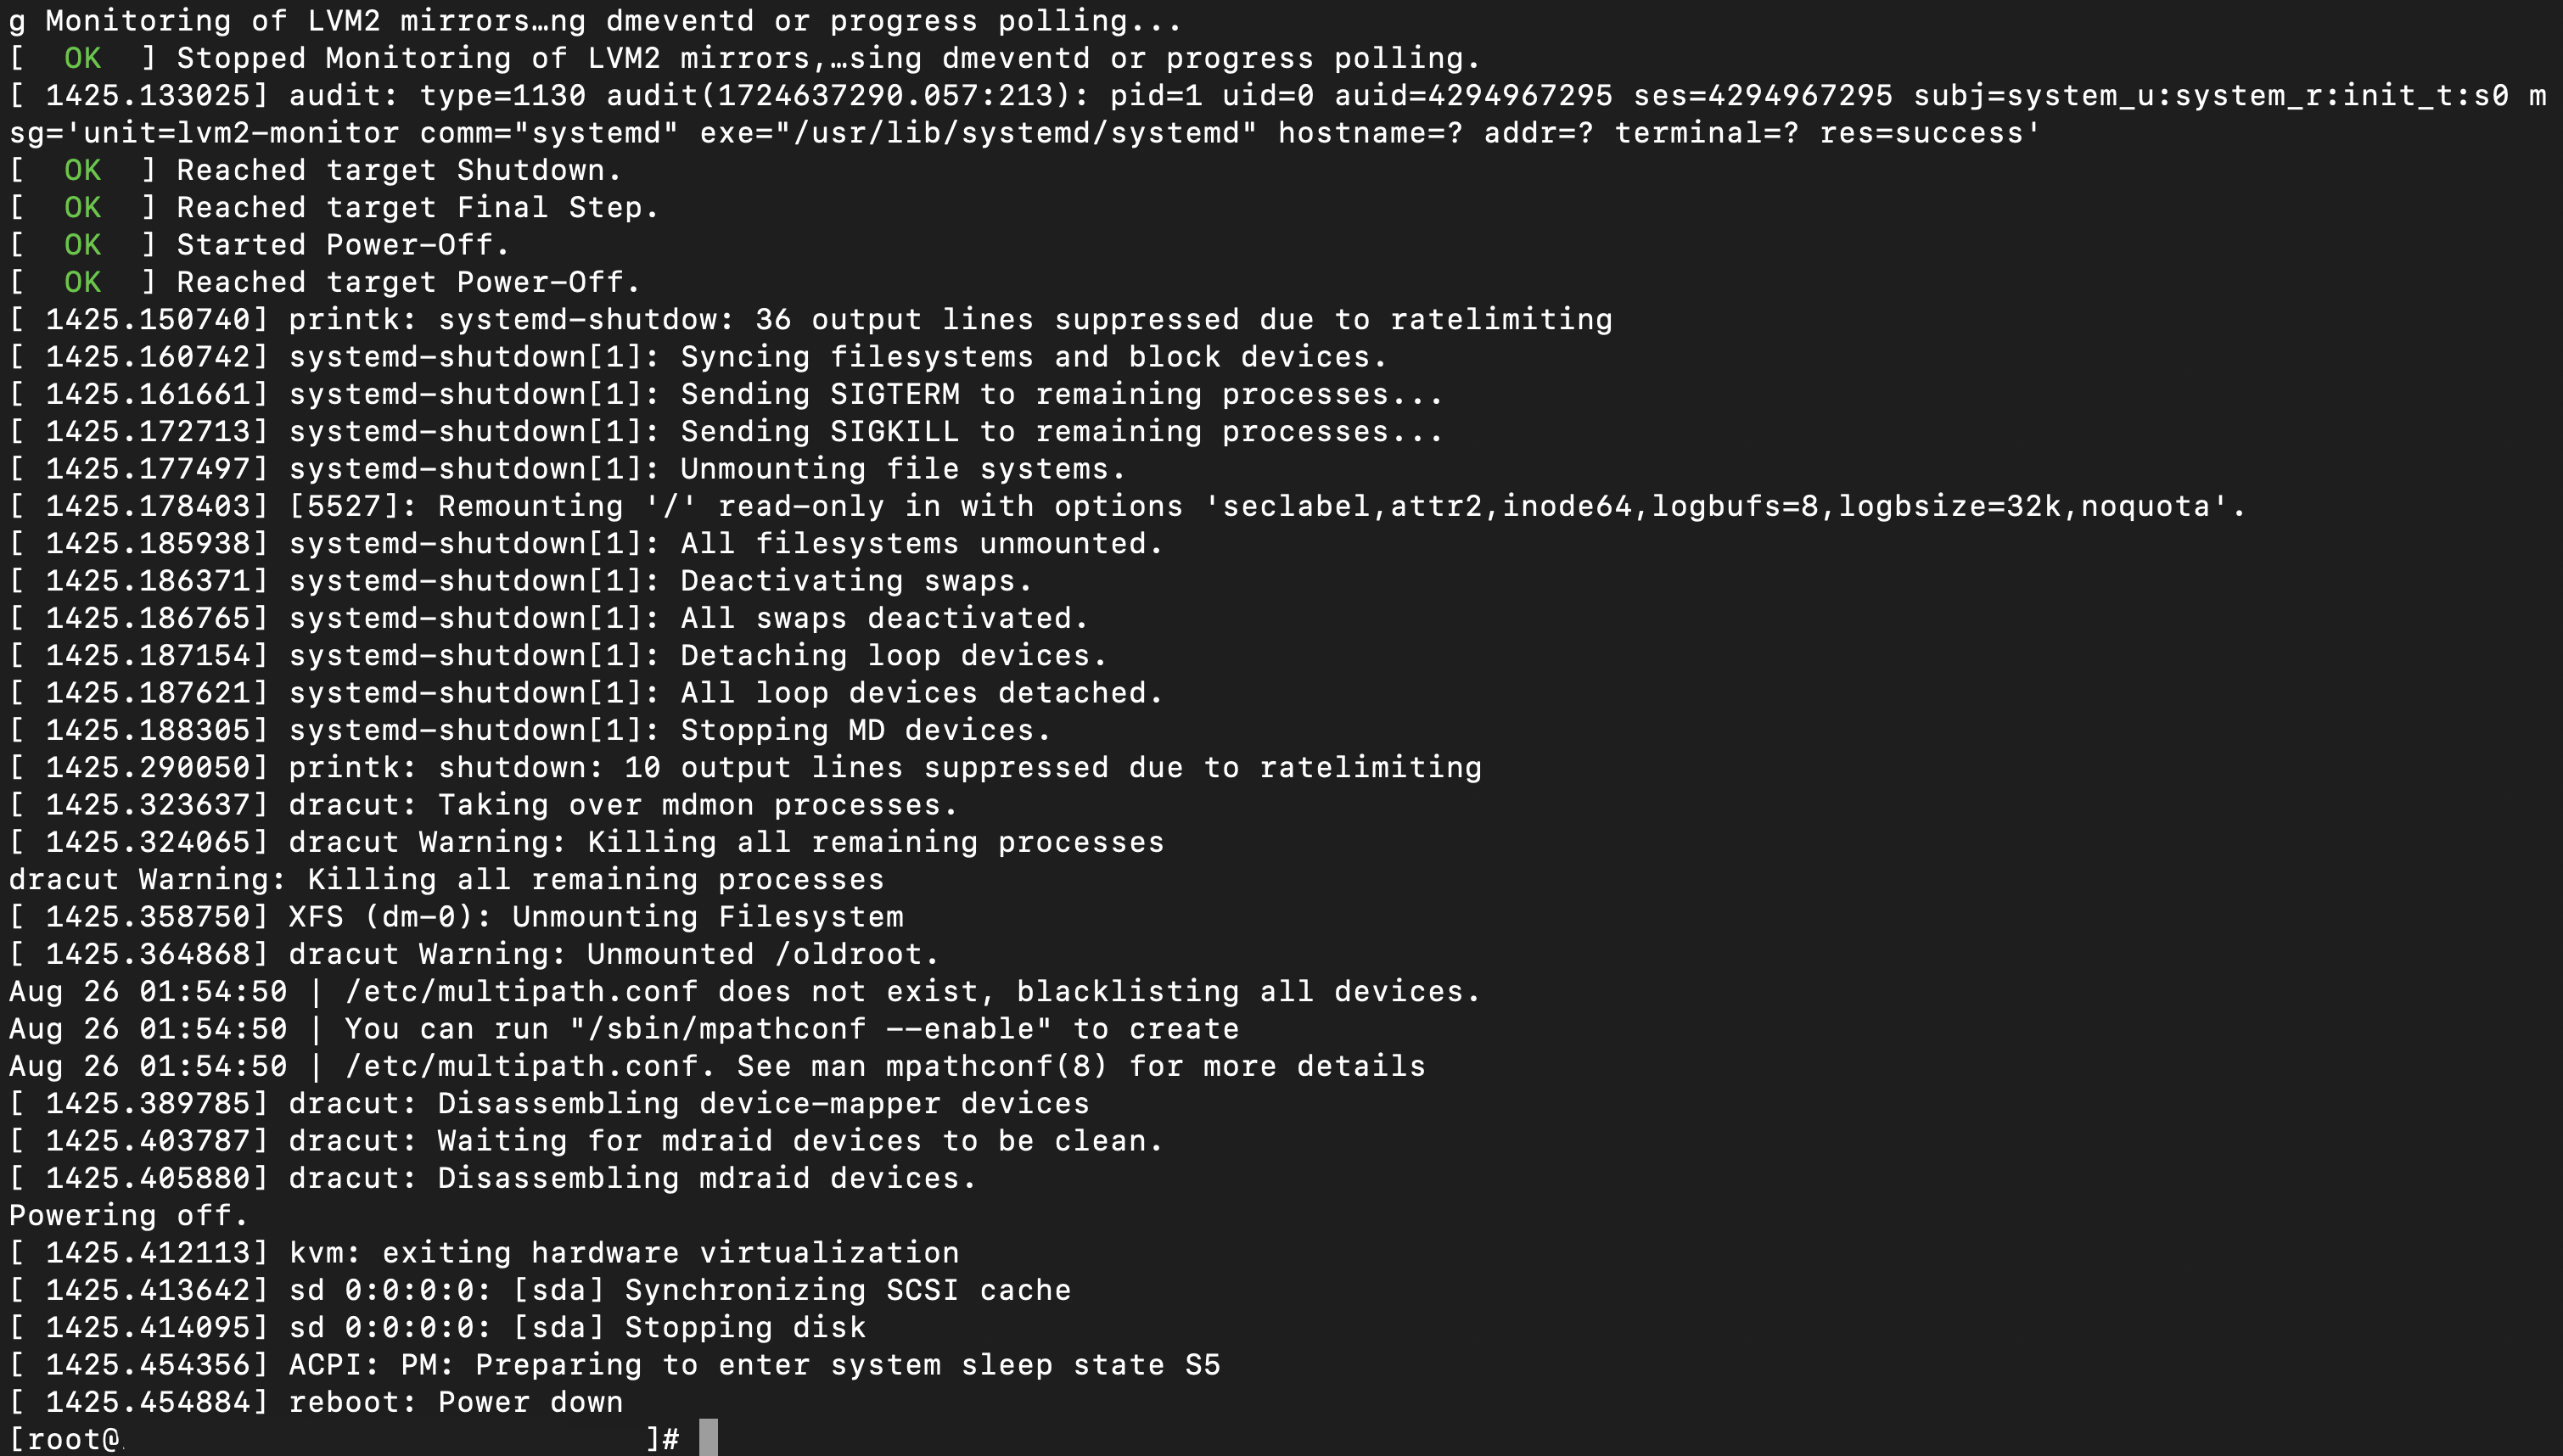
\includegraphics[width=\linewidth]{Images/Output of shutdowing guest.png}
              \captionof{figure}{Verification of Shutdown Process in the Guest}
              \label{fig:areboot}
          \end{center}
          The guest VM performed a clean shutdown, with all services stopping gracefully and the machine powering off as expected.
\end{itemize}

%% Some VNIC Hotplug/Unplug
\subsubsection[Some VNIC Hotplug/Unplug]{Some VNIC Hotplug/Unplug}
One of the critical tests involved the hotplug and unplug of VNICs. This test simulates scenarios where a high number of network interfaces are dynamically added and removed from the VM, which is common in environments that require high networking throughput and flexibility.\mynewline

Before starting the test, the existing network interfaces in the VM were listed using the ip a command to establish a baseline:
\begin{center}
    \centering
    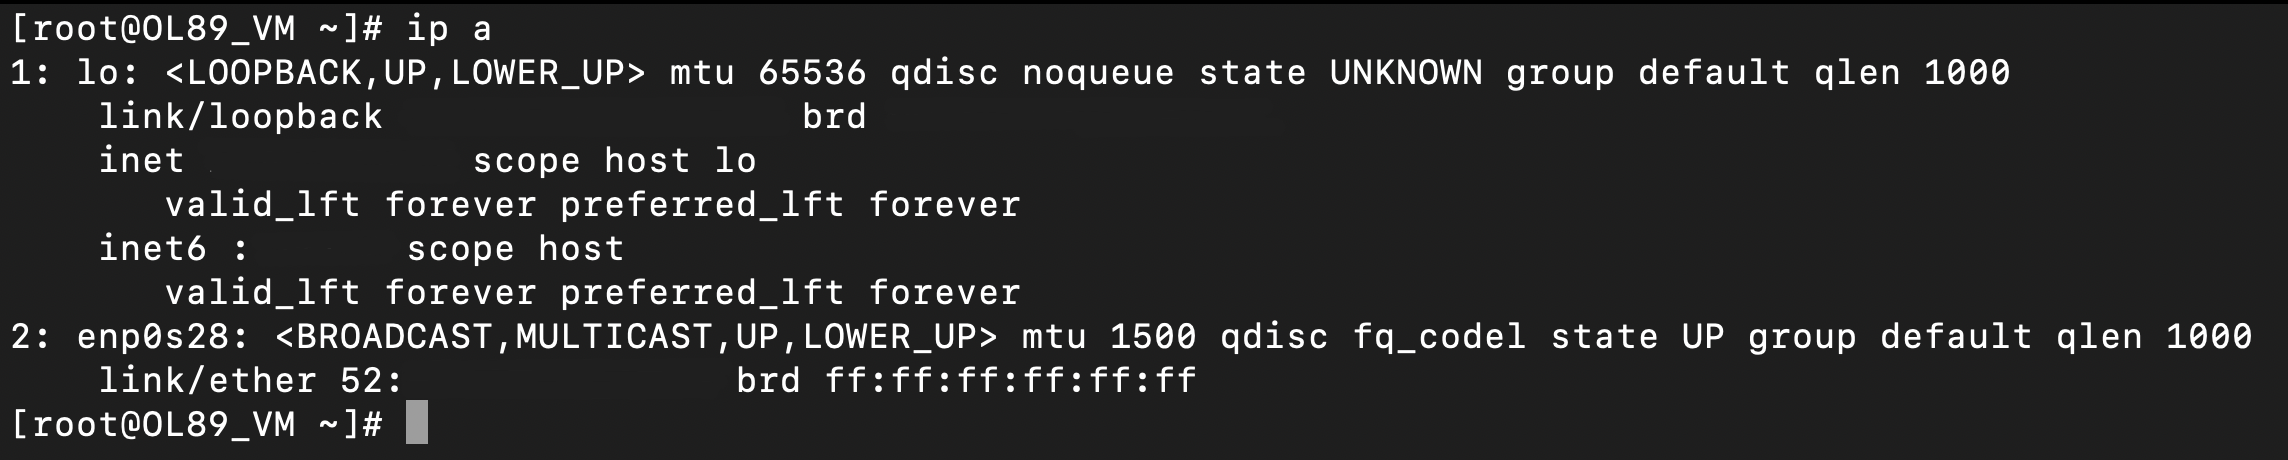
\includegraphics[width=\textwidth]{Images/Result of ip a.png}
    \captionof{figure}{Baseline Network Interface Configuration in the Guest}
    \label{fig}
\end{center}

A custom script, VNIC\_Hotplug.sh, was developed to automate the process of adding and removing VNICs. This script used QEMU monitor commands to systematically add VNICs to the running VM, simulating a high-density networking environment.

\begin{center}
    \centering
    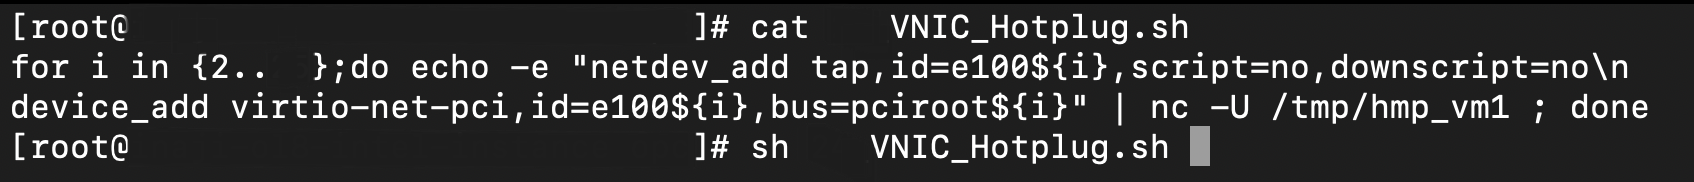
\includegraphics[width=\textwidth]{Images/24 VNIC Hotplug Script.png}
    \captionof{figure}{Executing VNIC Hotplug Script}
    \label{fig}
\end{center}

During the hotplug process, each new VNIC was detected by the guest, with appropriate entries appearing in the system logs (dmesg) and the network configuration being updated dynamically.\mynewline

The script iterated through each VNIC, ensuring that all interfaces were added without causing instability or significant performance degradation.\mynewline

After the VNICs were added, the ip a command was run again to confirm that all interfaces were successfully hotplugged:

\begin{center}
    \centering
    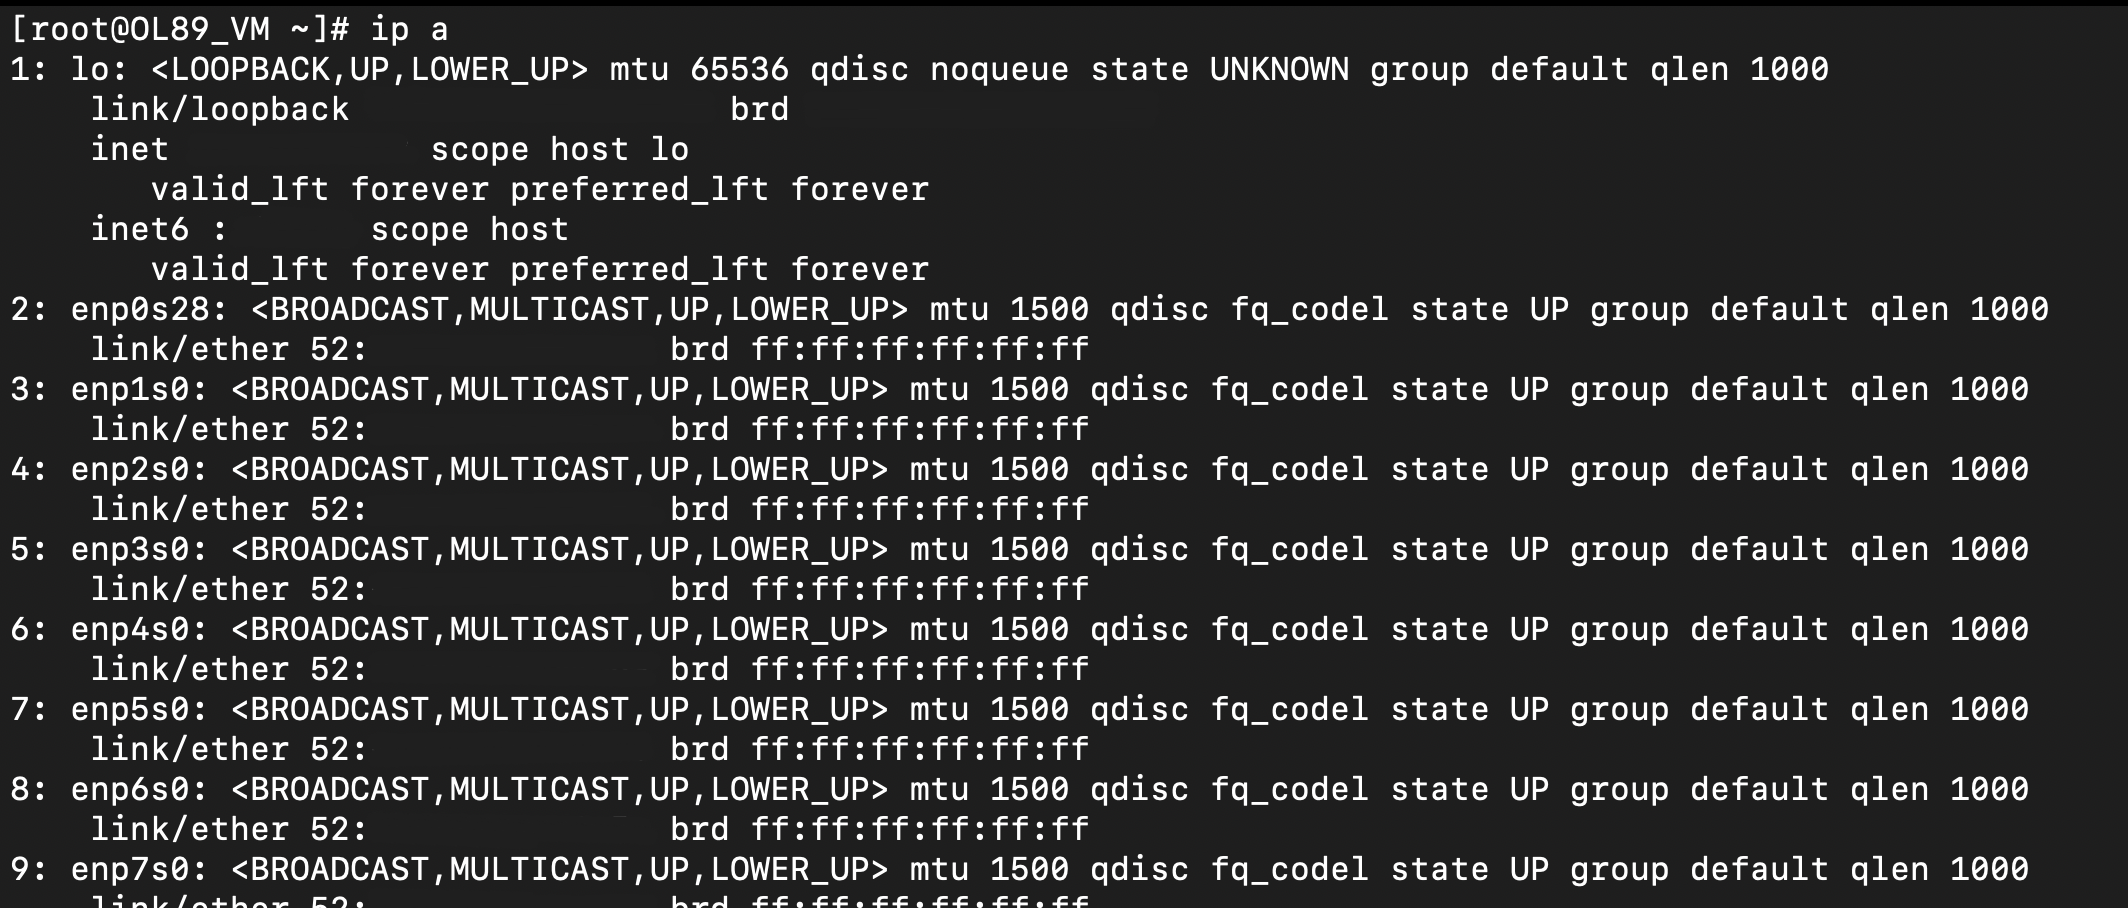
\includegraphics[width=\textwidth]{Images/VNIC result ip a (1).png}
    \captionof{figure}{Post-Hotplug Network Interface List in the Guestgit}
    \label{fig}
\end{center}
\noindent
\mynewline
Each VNIC was successfully added and configured, indicating that the VM's networking stack is robust and capable of handling dynamic changes in network configuration.\mynewline

For the unplug process. The script then proceeded to remove each VNIC one by one, ensuring that the system could handle the removal process without any issues. The VM continued to operate normally, and the removal of VNICs was verified by checking the updated network interface list.
\begin{center}
    \centering
    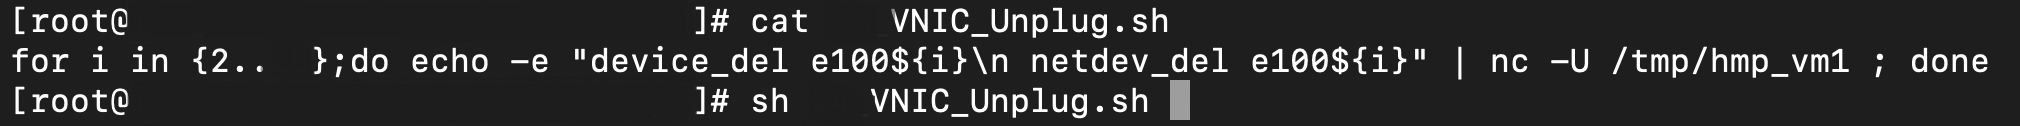
\includegraphics[width=\textwidth]{Images/24 VNIC Unplug Script.png}
    \captionof{figure}{Executing VNIC Unplug Script}
    \label{fig}
\end{center}
\begin{center}
    \centering
    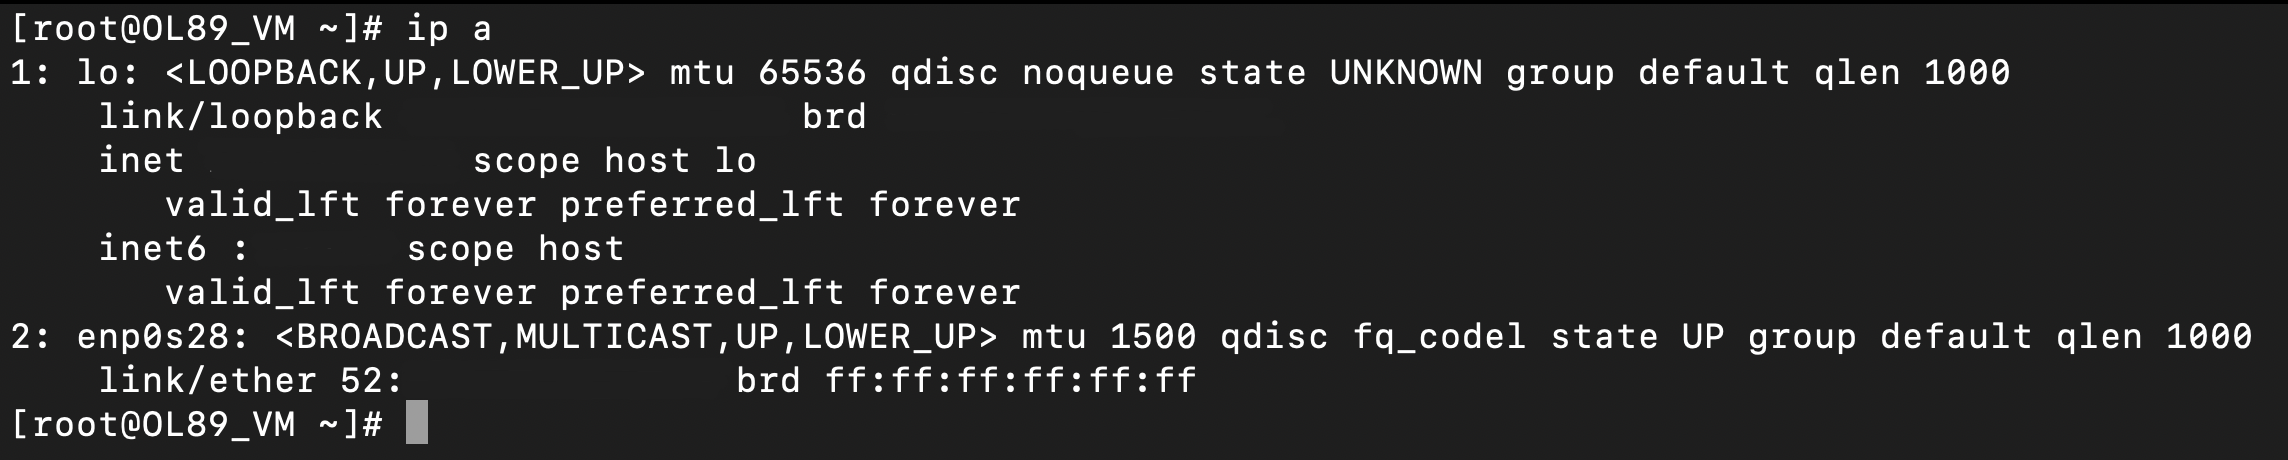
\includegraphics[width=\textwidth]{Images/Result of ip a.png}
    \captionof{figure}{Updated Network Interface List After VNIC Unplug}
    \label{fig}
\end{center}


%% VFIO-VNIC Hotplug/Unplug
\subsubsection[Some VFIO-VNIC Hotplug/Unplug]{Some VFIO-VNIC Hotplug/Unplug}
For this test, the process involved the creation and management of some VFIO VNICs on the host system. The initial step required preparing the VFIO VNICs to be bound to the host, ensuring that they were correctly set up for use in the virtualization environment. This involved configuring the VFIO devices so they could be utilized by the guest VM.

\begin{center}
    \centering
    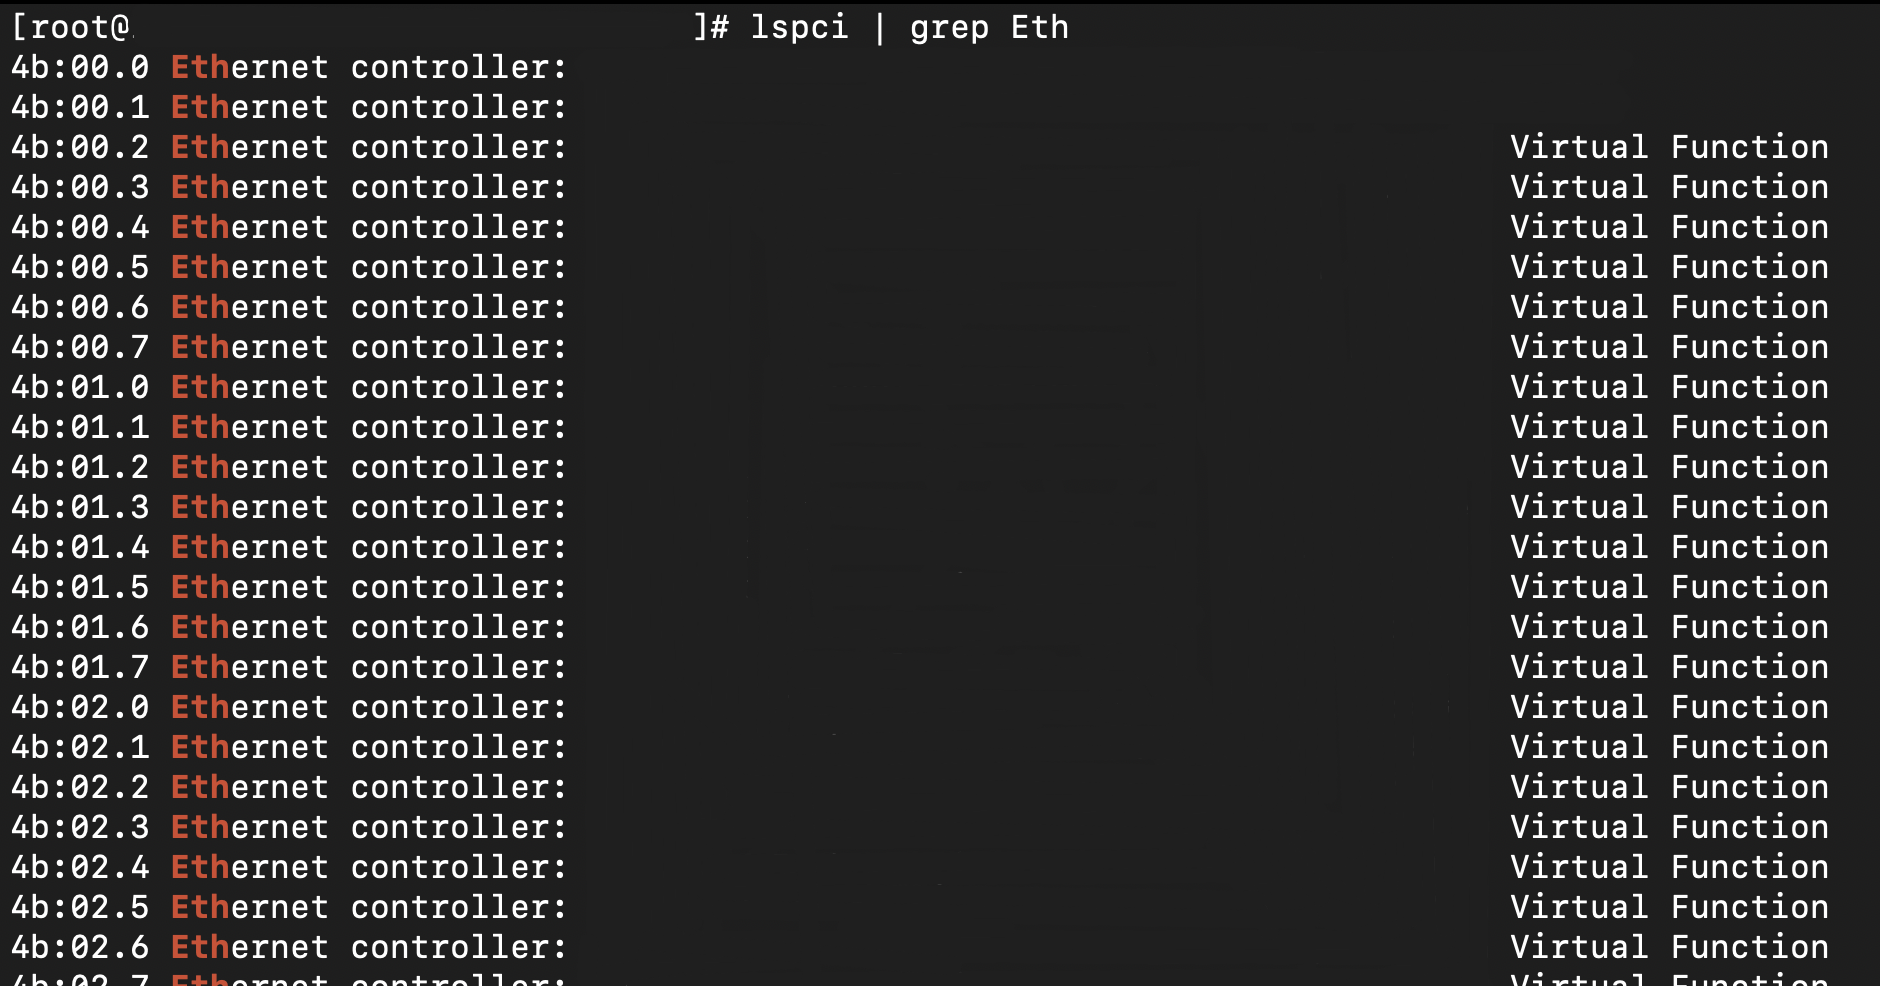
\includegraphics[width=\textwidth]{Images/LSPCI Grep ETh.png}
    \captionof{figure}{Listing PCI Devices Bound to VFIO on Host}
    \label{fig}
\end{center}

Once the VFIO VNICs were set up, the hotplug process was initiated. The script for adding VFIO-VNICs to the VM is as follows:

\begin{center}
    \centering
    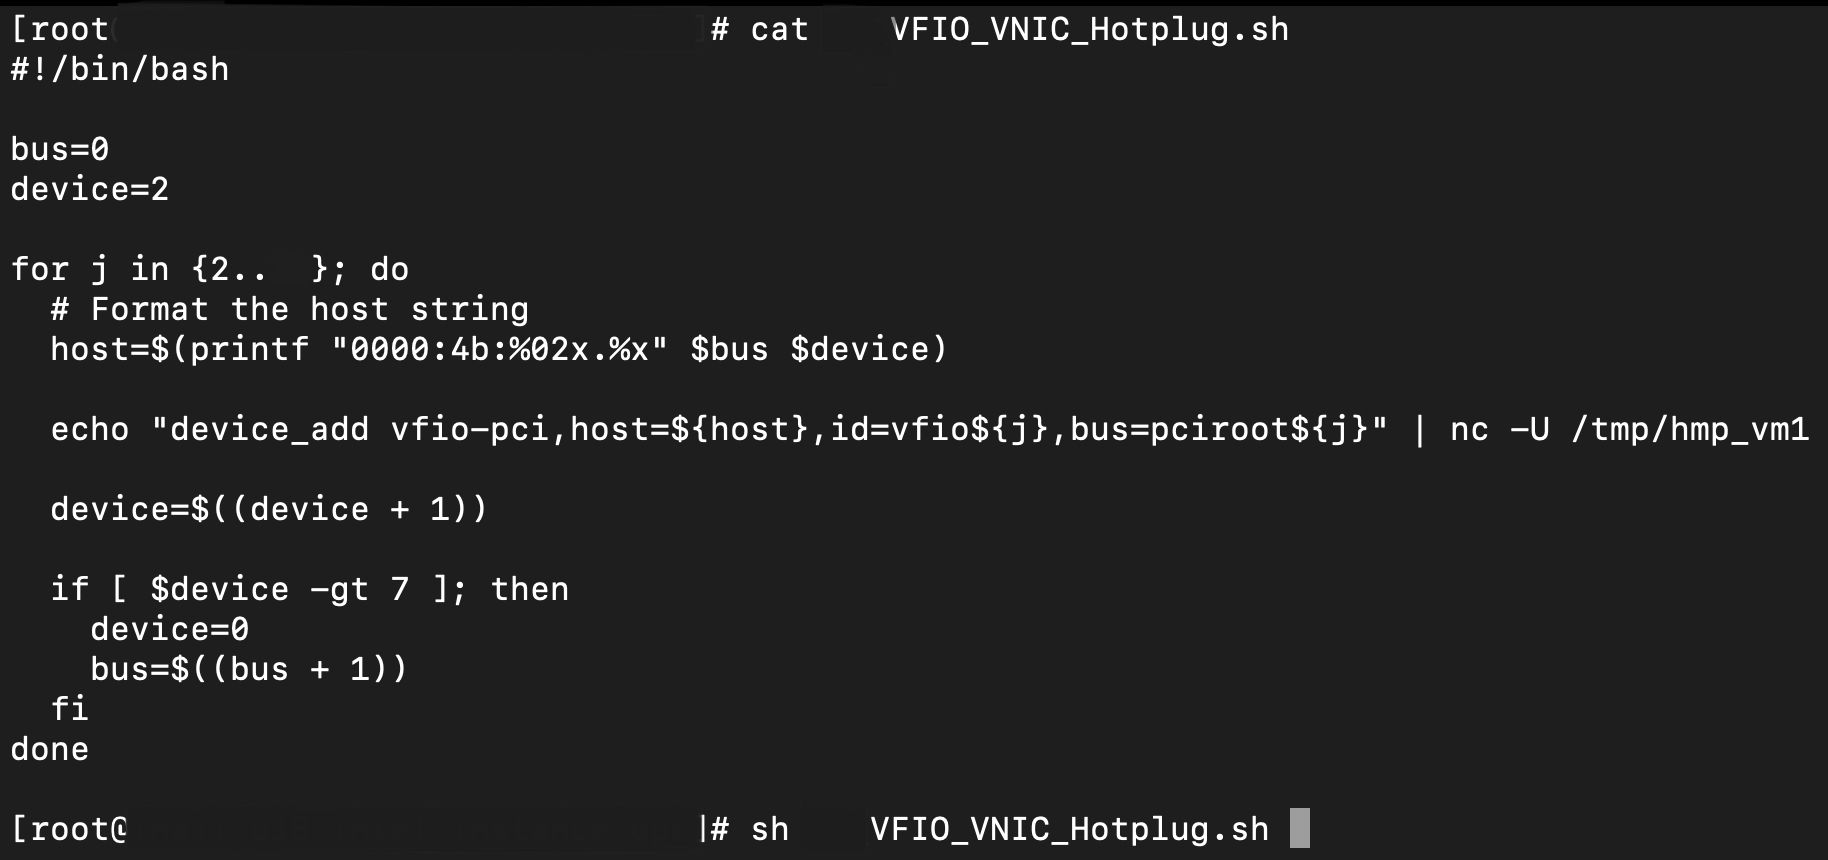
\includegraphics[width=\textwidth]{Images/24 VFIO VNIC Hotplug Script.png}
    \captionof{figure}{Executing VFIO VNIC Hotplug Script}
    \label{fig}
\end{center}

This script systematically adds VFIO VNICs to the VM by sending commands to the QEMU monitor to attach each device. Each VNIC was successfully detected by the guest VM, as confirmed by the updated network interface list after the hotplug operation.

\begin{center}
    \centering
    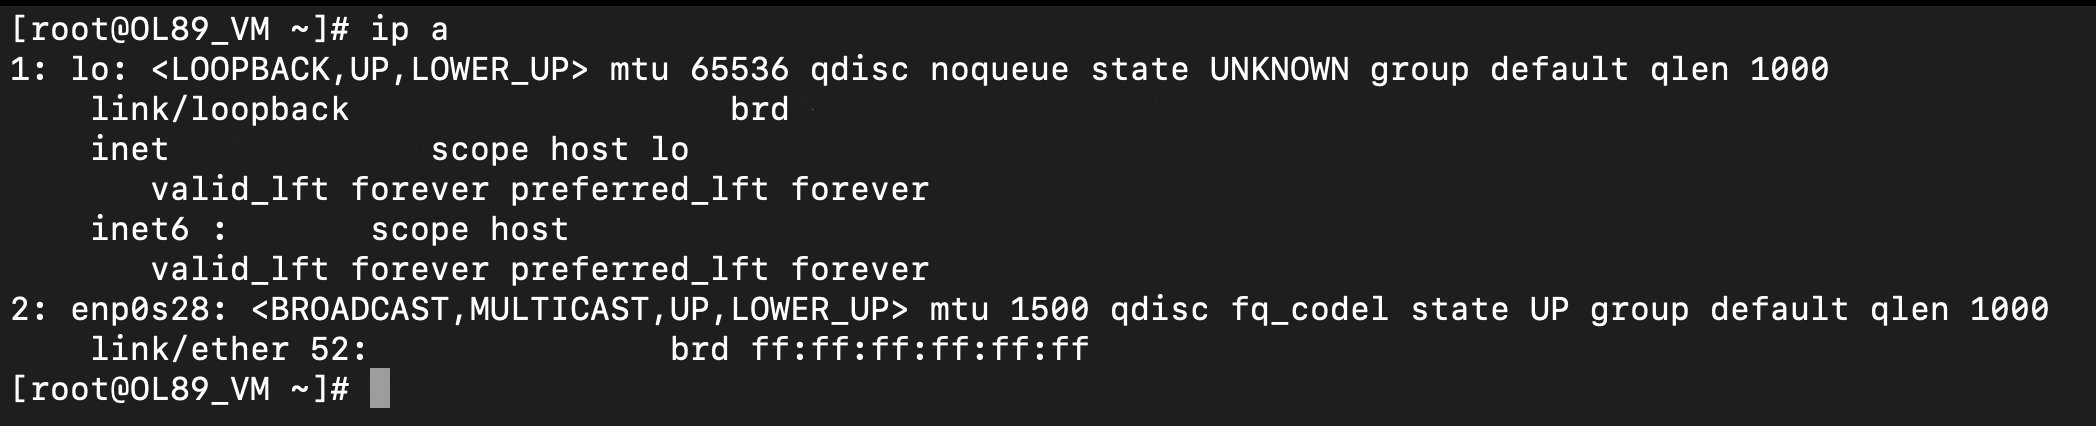
\includegraphics[width=\textwidth]{Images/ip a before hotplug vfio.png}
    \captionof{figure}{Network Interface List Before VFIO VNIC Hotplug}
    \label{fig}
\end{center}

\begin{center}
    \centering
    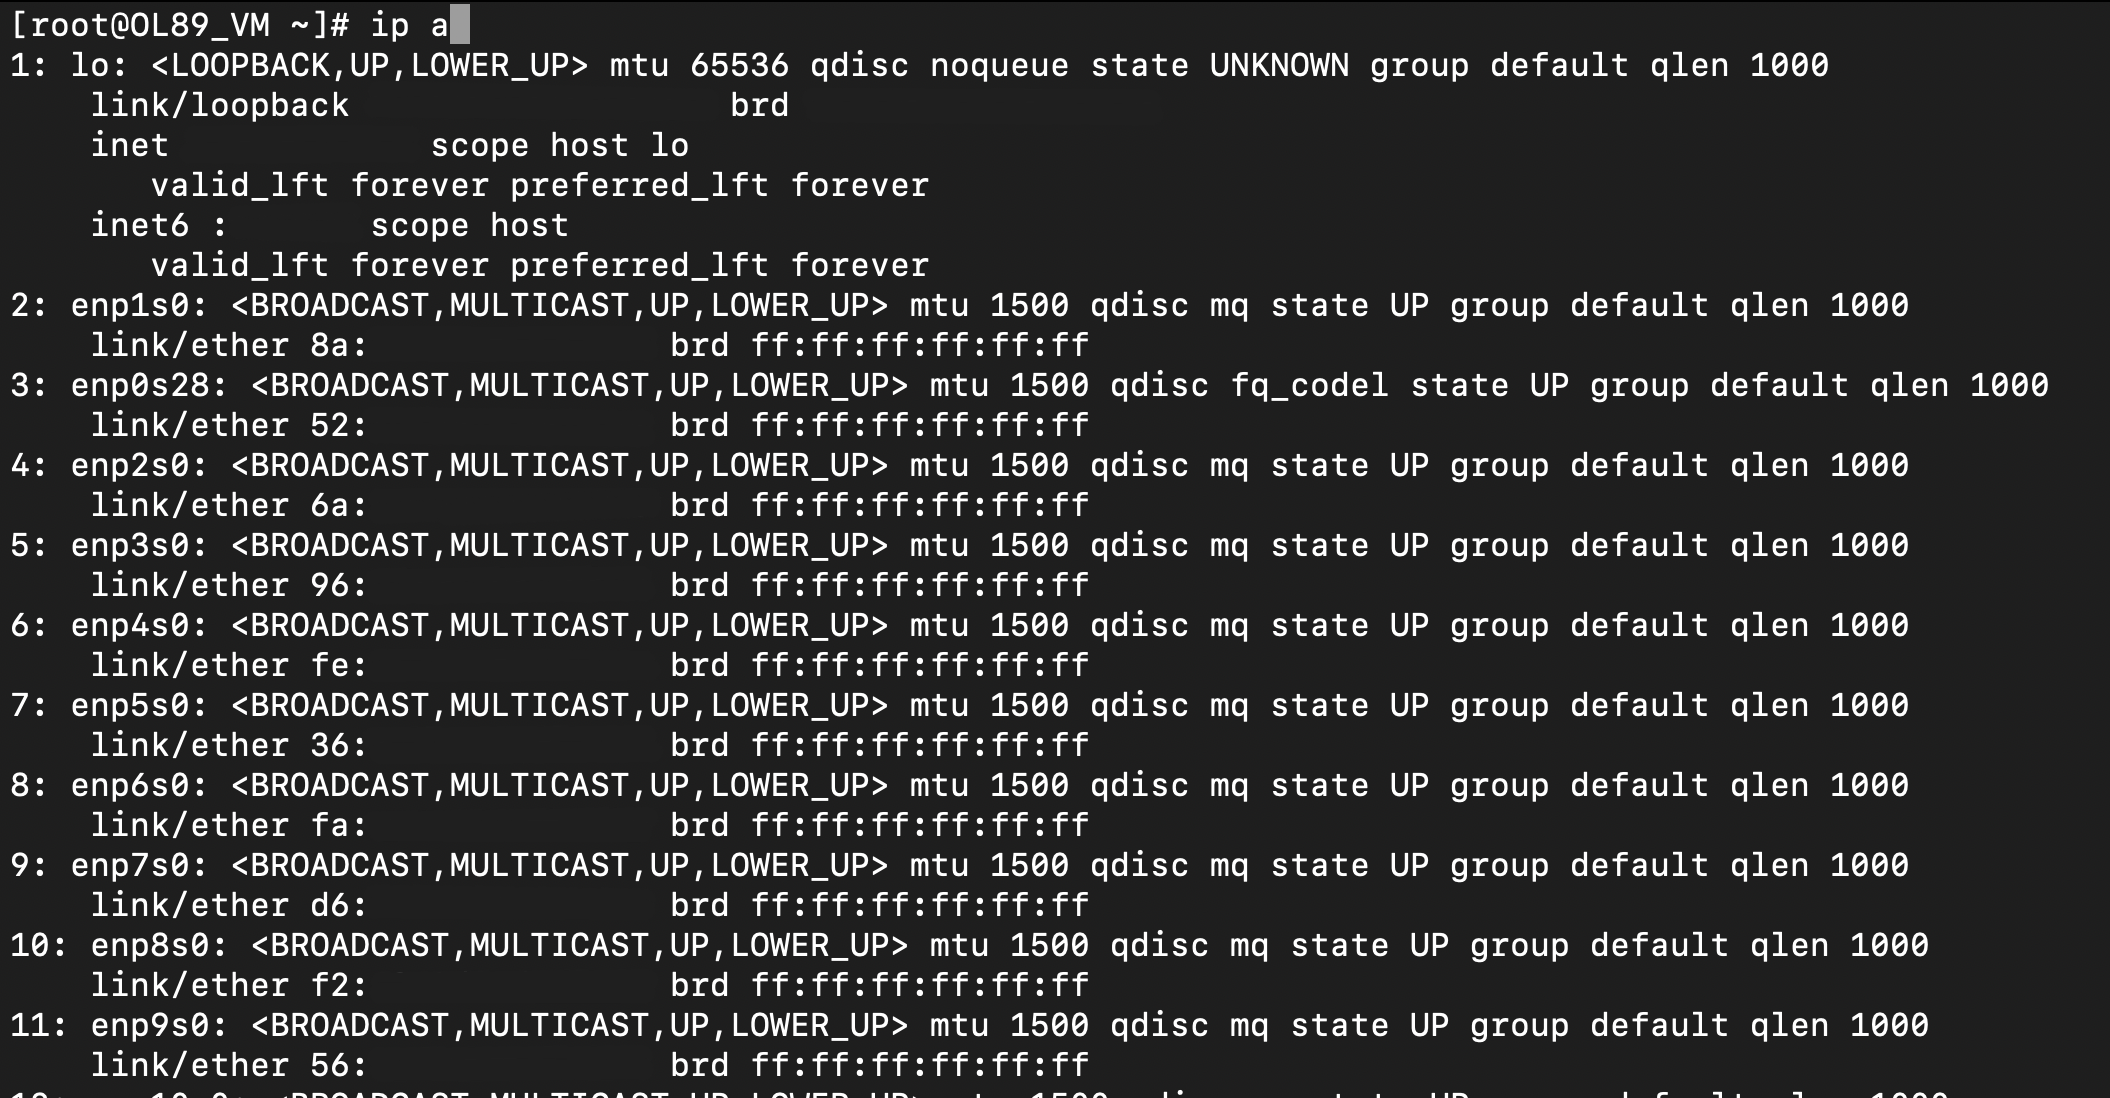
\includegraphics[width=\textwidth]{Images/ip a after vfio.png}
    \captionof{figure}{Post-Hotplug Network Interface List in Guest VM}
    \label{fig}
\end{center}

The verification involved checking the network interfaces before and after the hotplug, which showed all VNICs were added successfully. The guest VM maintained stable network operations, and the hotplug persisted after a reboot.\mynewline

For the unplug process, a different script was used:

\begin{center}
    \centering
    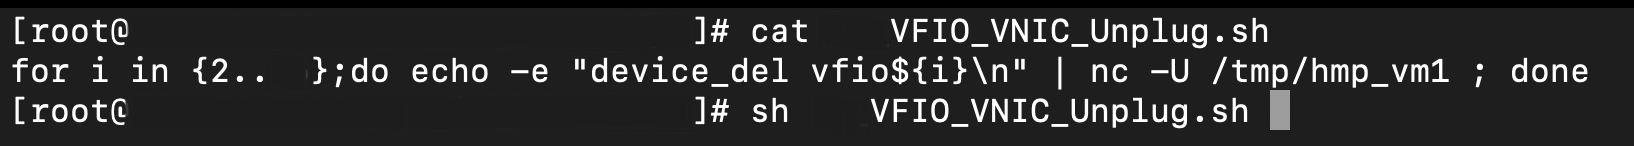
\includegraphics[width=\textwidth]{Images/24 VFIO VNIC Unplug Script.png}
    \captionof{figure}{Executing VFIO VNIC Unplug Script}
    \label{fig}
\end{center}

This script removes the VFIO VNICs one by one by sending commands to the QEMU monitor. After unplugging the VNICs, the network interface list was checked to ensure the removal was successful. The guest VM continued to operate normally, and the network configuration was updated accordingly.

\begin{center}
    \centering
    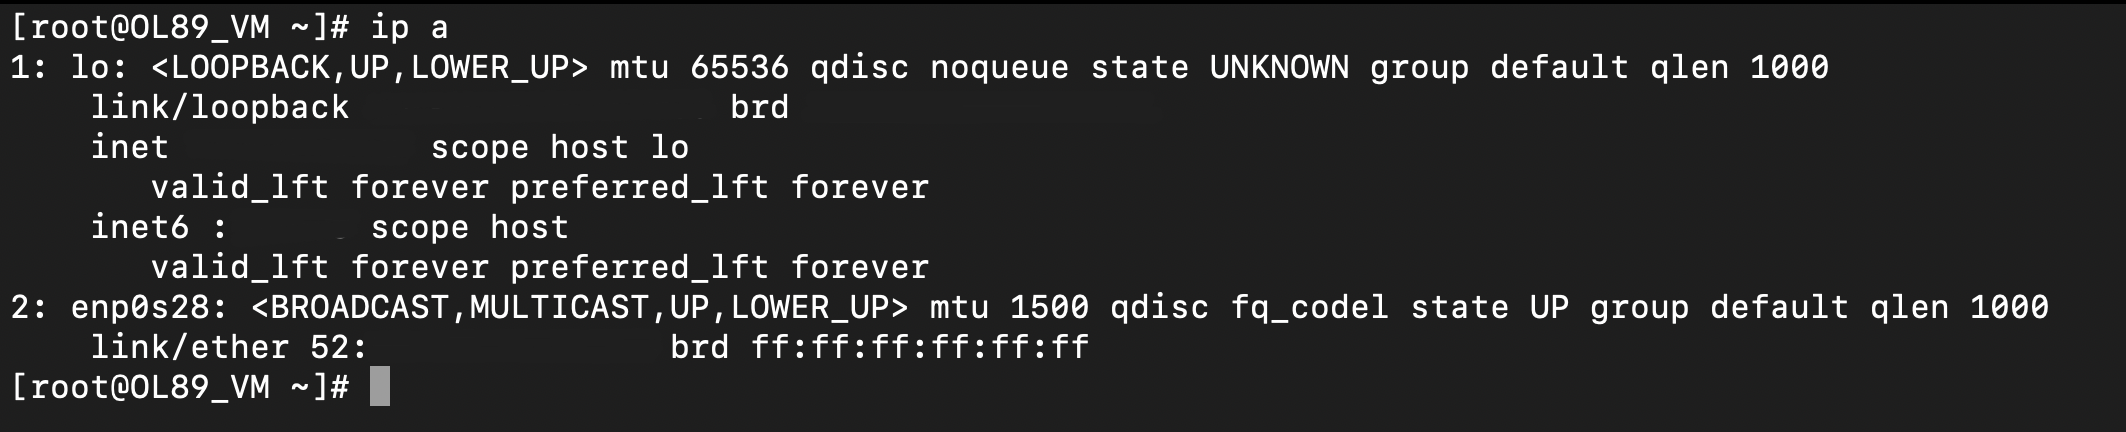
\includegraphics[width=\textwidth]{Images/ip a after VFIO Unplug.png}
    \captionof{figure}{Updated Network Interface List After VFIO VNIC Unplug}
    \label{fig}
\end{center}


%% VDisk Hotplug/Unplug
\subsubsection[VDisks Hotplug/Unplug]{VDisks Hotplug/Unplug}
For this test, we prepared some virtual disk images on the host system. The creation of these disk images was accomplished with the following commands:

\begin{center}
    \centering
    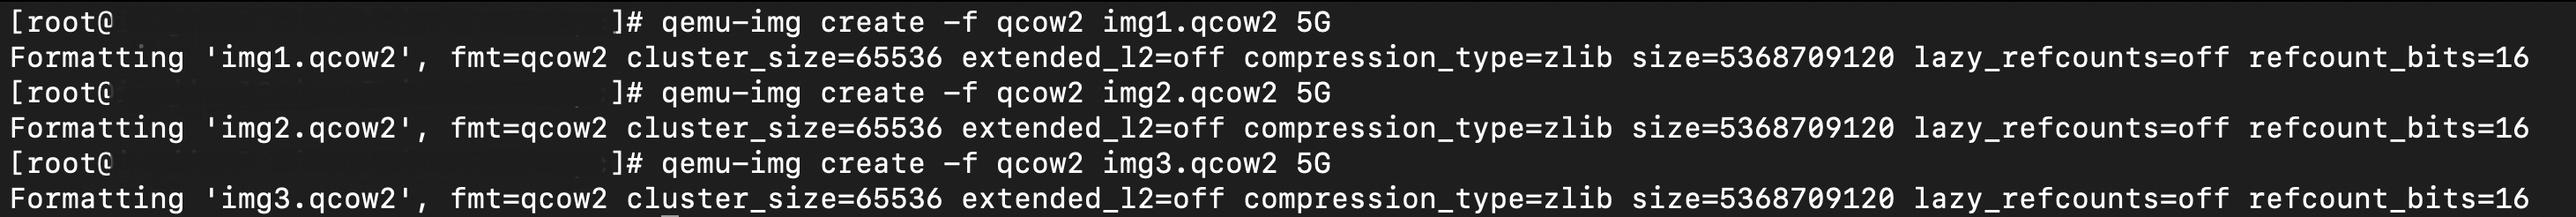
\includegraphics[width=\textwidth]{Images/Creating 3 vDisks.png}
    \captionof{figure}{Creating vDisks on Host System}
    \label{fig}
\end{center}

These commands generated three 5GB disk images in QCOW2 format, which were then used for hotplug testing.\mynewline

The hotplug process involved adding these virtual disks to the VM using the following QEMU monitor commands:

\begin{center}
    \centering
    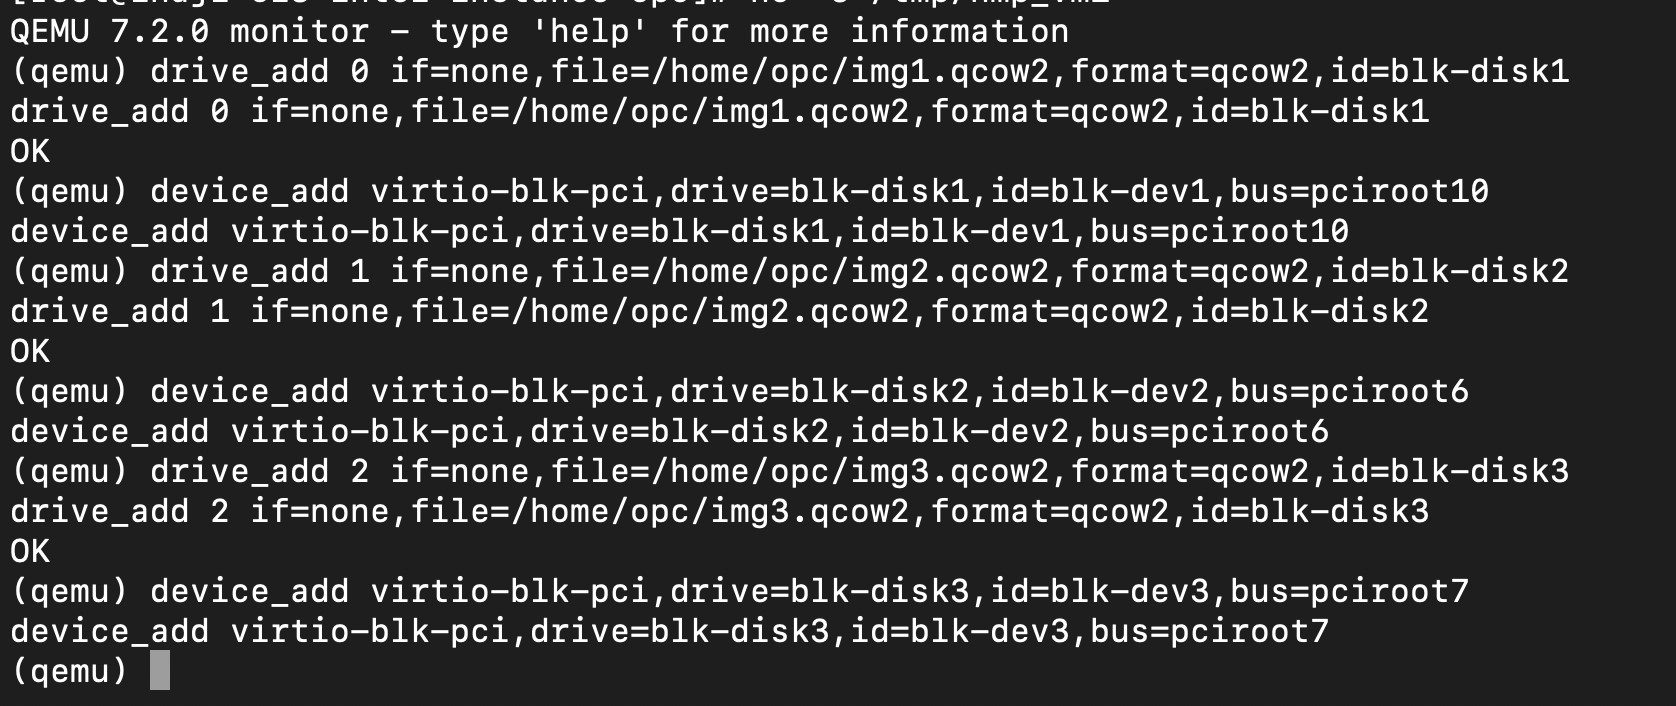
\includegraphics[width=\textwidth]{Images/3 vDisk Hotplug.png}
    \captionof{figure}{Hotplugging vDisks Command Sequence}
    \label{fig}
\end{center}

Before initiating the hotplug, the lsblk command was used to display the existing block devices:

\begin{center}
    \centering
    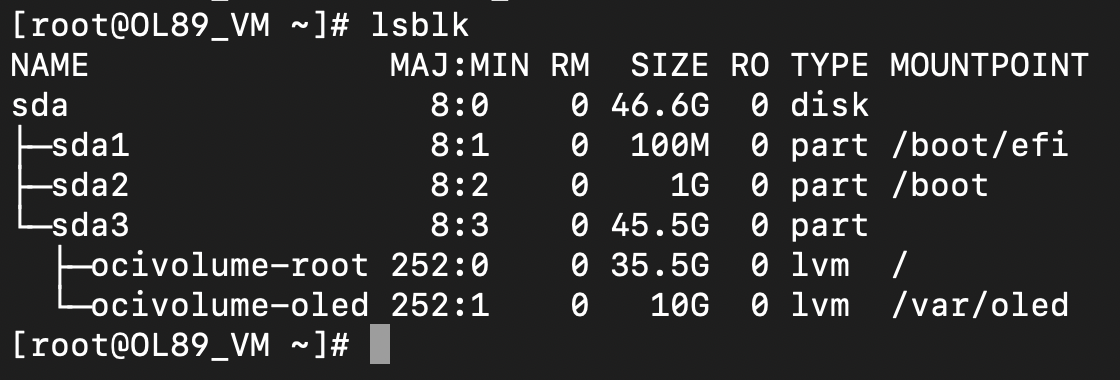
\includegraphics[width=\textwidth]{Images/lsblk before hotplug.png}
    \captionof{figure}{Block Device List Before vDisks Hotplug}
    \label{fig}
\end{center}

During the hotplug, new entries appeared in the system logs, indicating that the disks were successfully detected and attached. After the hotplug, running lsblk again showed the new disks:

\begin{center}
    \centering
    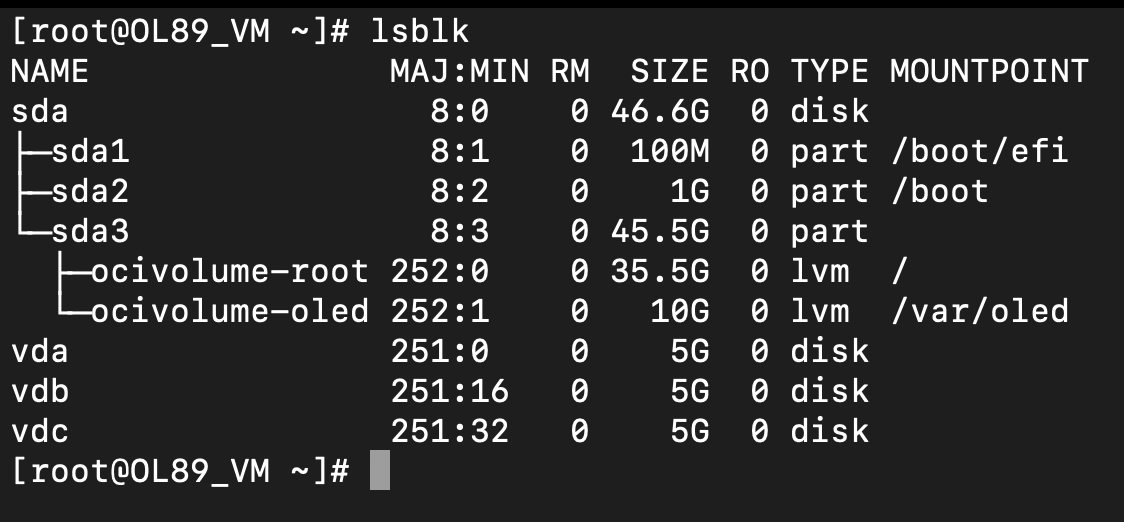
\includegraphics[width=\textwidth]{Images/lsblk after hotplug.png}
    \captionof{figure}{Block Device List After vDisks Hotplug}
    \label{fig}
\end{center}

The new disks were listed correctly, confirming the success of the hotplug operation.\mynewline

For the unplug test, the disks were removed using similar QEMU monitor commands. This process was confirmed by checking the lsblk output again, which showed the disks were no longer present, verifying that the unplug operation was successful.


%% Kdump Check
\subsubsection[Kdump Check]{Kdump Check}
To verify Kdump functionality, we configured the system to capture crash dumps during kernel failures. This involved setting up the \texttt{/etc/kdump.conf} file to designate a local dump directory and specifying memory allocation for dump files. We checked the Kdump service status with the command \texttt{systemctl status kdump.service} to ensure it was active.\mynewline

To test the setup, a kernel panic was induced using \texttt{echo c > /proc/sysrq-trigger}, causing the system to reboot. Upon restart, we verified that dump files were present in \texttt{/var/oled/crash}.

\begin{center}
    \centering
    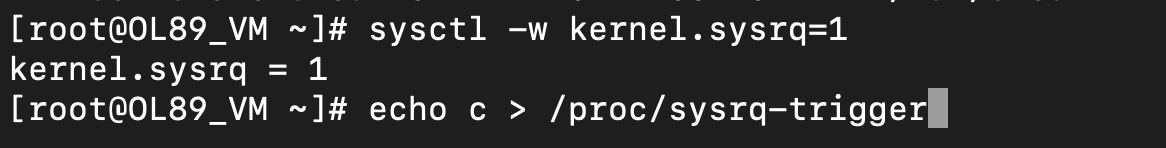
\includegraphics[width=\textwidth]{Images/Launch Kdump.png}
    \captionof{figure}{Initiating Kdump Process}
    \label{fig}
\end{center}

\begin{center}
    \centering
    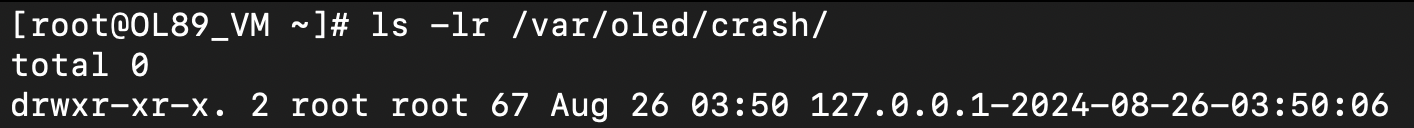
\includegraphics[width=\textwidth]{Images/Crash Folder.png}
    \captionof{figure}{Crash Dump Directory Verification}
    \label{fig}
\end{center}

Analysis tools such as crash were used to inspect the dump files, confirming that Kdump was correctly capturing crash data.


%% Memory Hotplug/Unplug
\subsubsection[Memory Hotplug/Unplug]{Memory Hotplug/Unplug}
The memory hotplug/unplug test was conducted to assess the VM’s capability to dynamically add and remove memory. Initially, we aimed to add 16 GB of memory to the guest VM using QEMU commands. The following QEMU monitor commands were used to add memory:

\begin{center}
    \centering
    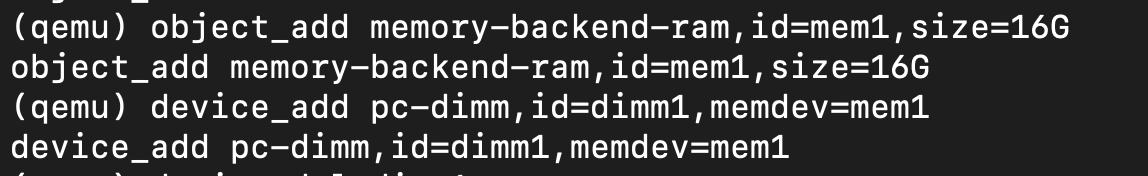
\includegraphics[width=\textwidth]{Images/Memory Hotplug.png}
    \captionof{figure}{Executing Memory Hotplug Process}
    \label{fig}
\end{center}

Before initiating the test, we checked the VM's current memory configuration with the lsmem command:

\begin{center}
    \centering
    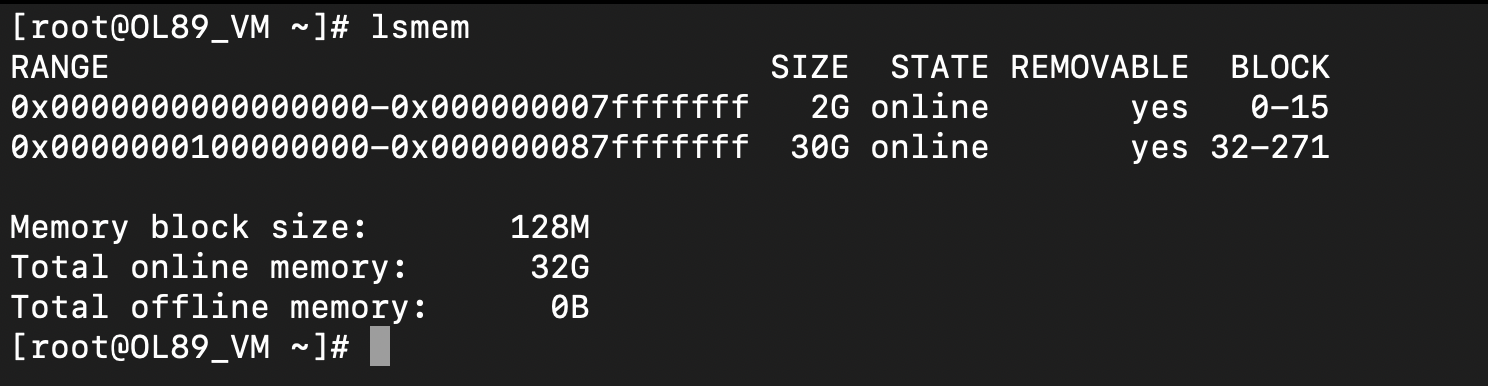
\includegraphics[width=\textwidth]{Images/lsmem after unplug.png}
    \captionof{figure}{Memory Status Before the Hotplugging}
    \label{fig}
\end{center}

After the addition, the lsmem command showed the following updated memory configuration:

\begin{center}
    \centering
    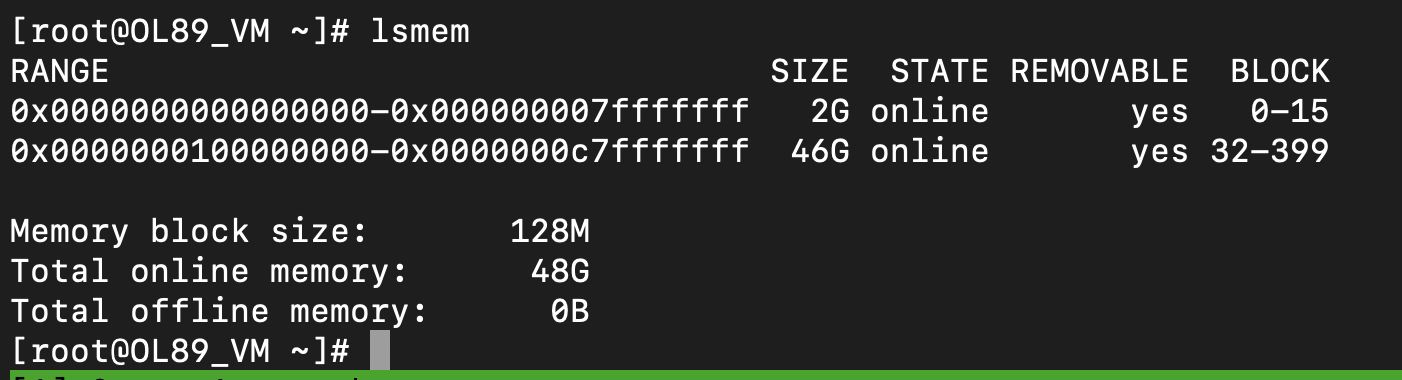
\includegraphics[width=\textwidth]{Images/lsmem after hotplug.png}
    \captionof{figure}{Memory Status After Hotplugging}
    \label{fig}
\end{center}

After a reboot, the memory configuration remained at 48 GB, confirming that the hotplug operation was successful.\mynewline

For the memory unplug test, the following QEMU monitor commands were used:

\begin{center}
    \centering
    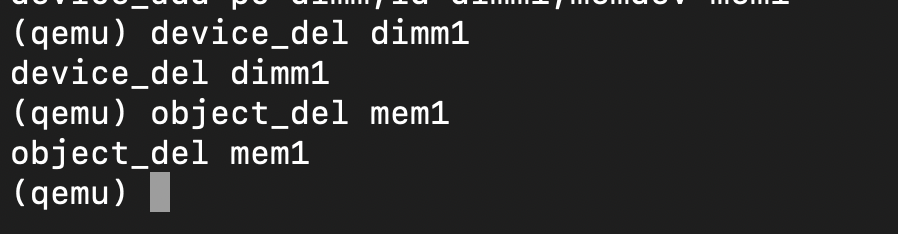
\includegraphics[width=\textwidth]{Images/Memory Unplug.png}
    \captionof{figure}{Executing Memory Unplug Process}
    \label{fig}
\end{center}

Post-unplug, the memory configuration reverted to its initial state:

\begin{center}
    \centering
    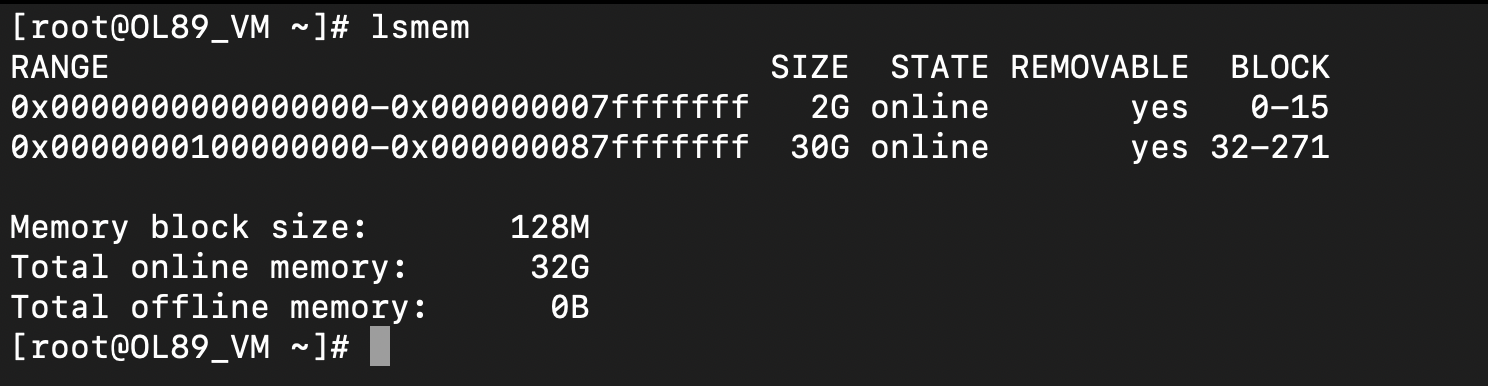
\includegraphics[width=\textwidth]{Images/lsmem after unplug.png}
    \captionof{figure}{Memory Status After Unplugging}
    \label{fig}
\end{center}



%% Overview of Testing Outcomes
\subsubsection[Overview of Testing Outcomes]{Overview of Testing Outcomes}

In this section, we summarize the outcomes of the various tests conducted. The tests covered a range of functionalities, including lifecycle operations, hotplug/unplug of network interfaces, virtual disks, and memory. Each test aimed to validate the stability and performance of the VM in handling dynamic changes and typical operational states.\mynewline

Key findings from the tests include:

\begin{itemize}
    \item \textbf{Lifecycle Operations:} The VM successfully handled reboot, stop/continue, suspend, and shutdown operations without issues. The system remained stable and responsive through each state transition;
    \item \textbf{Hotplug/Unplug of VNICs:} Both standard and VFIO VNICs were tested. The guest VM efficiently managed the addition and removal of VNICs, demonstrating robustness in network interface handling;
    \item \textbf{VDisk Hotplug/Unplug:} The VM successfully attached and detached virtual disks, with the system recognizing new disks and removing them as expected;
    \item \textbf{Memory Hotplug/Unplug:} The VM handled the addition and removal of memory dynamically. The system maintained stability and correctly updated its memory configuration.
\end{itemize}

Performance metrics and system logs throughout the tests showed that the VM operated within expected parameters, confirming the effectiveness of the tested features and the stability of the virtual environment.

%% Manual sanity test with Qemu 7.2.0-14 oci AMD Host OL8+UEK7U2 Guest: OL 7.9 + UEK6U3
\section{Test on OL8 Host with an AMD CPU, QEMU and latest kernel version UEK6U3}

%% Host System and Guest VM Configuration 
\subsection{Host System and Guest VM Configuration}

For the second testing scenario, we utilized an AMD-based OCI Instance running Oracle Linux Server 8. This setup involved configuring the latest version of UEK7U2 on the host. The first step was to verify the installation and configuration of QEMU, ensuring that all components were correctly installed and the environment was properly set up.

The initial verification included checking the host system's configuration using the hostnamectl command, listing all relevant QEMU components, verifying the presence of edk2 packages:

\begin{center}
    \centering
    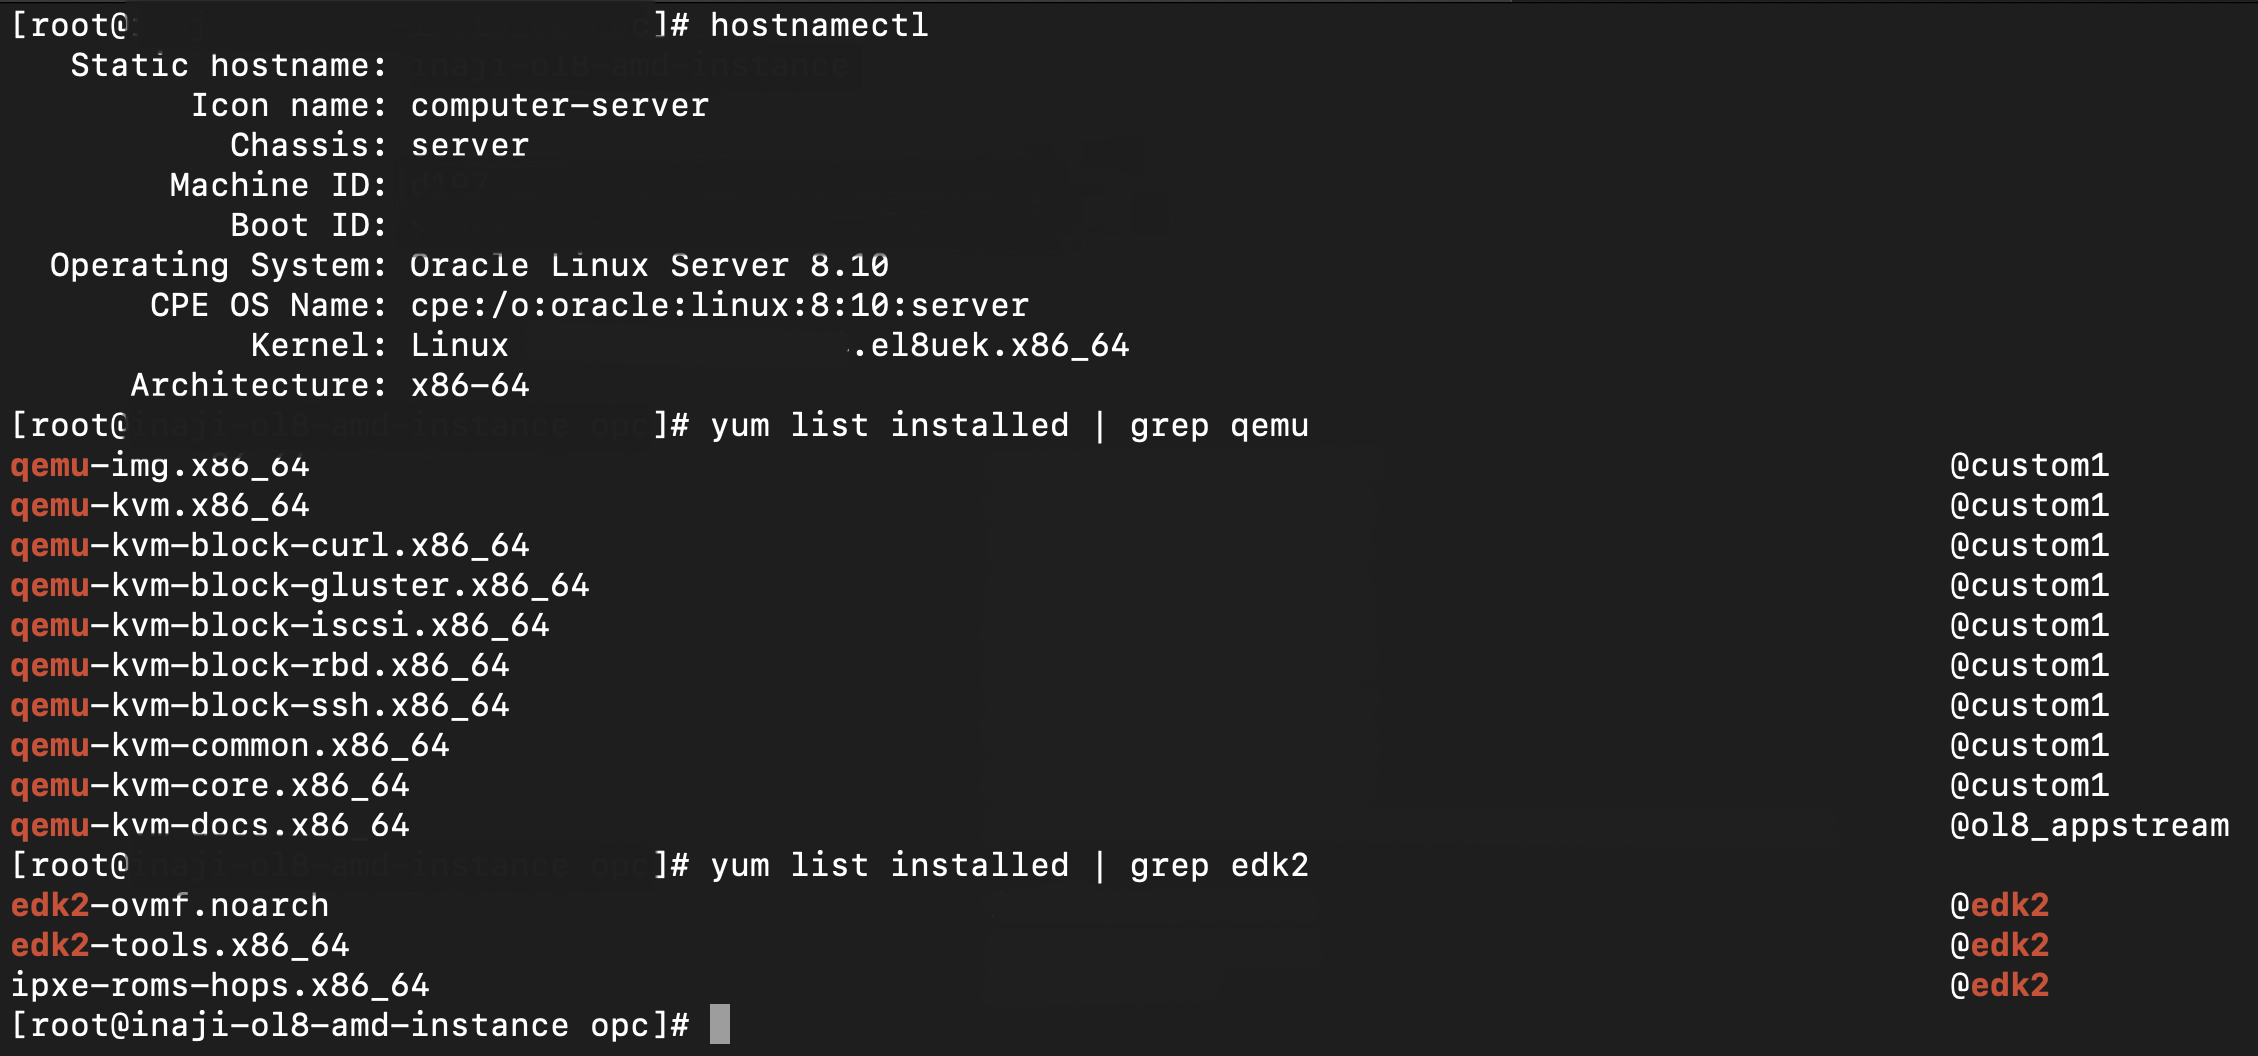
\includegraphics[width=\textwidth]{Images/Host System Configuration Verification.png}
    \captionof{figure}{Host System Configuration Verification}
    \label{fig:casa}
\end{center}

With the host system fully prepared, we proceeded to deploy the guest VM running Oracle Linux 7.9 with UEK6U3. The guest was initiated using the QEMU command which ensured that the guest VM was correctly set up for the testing phase:

\begin{center}
    \centering
    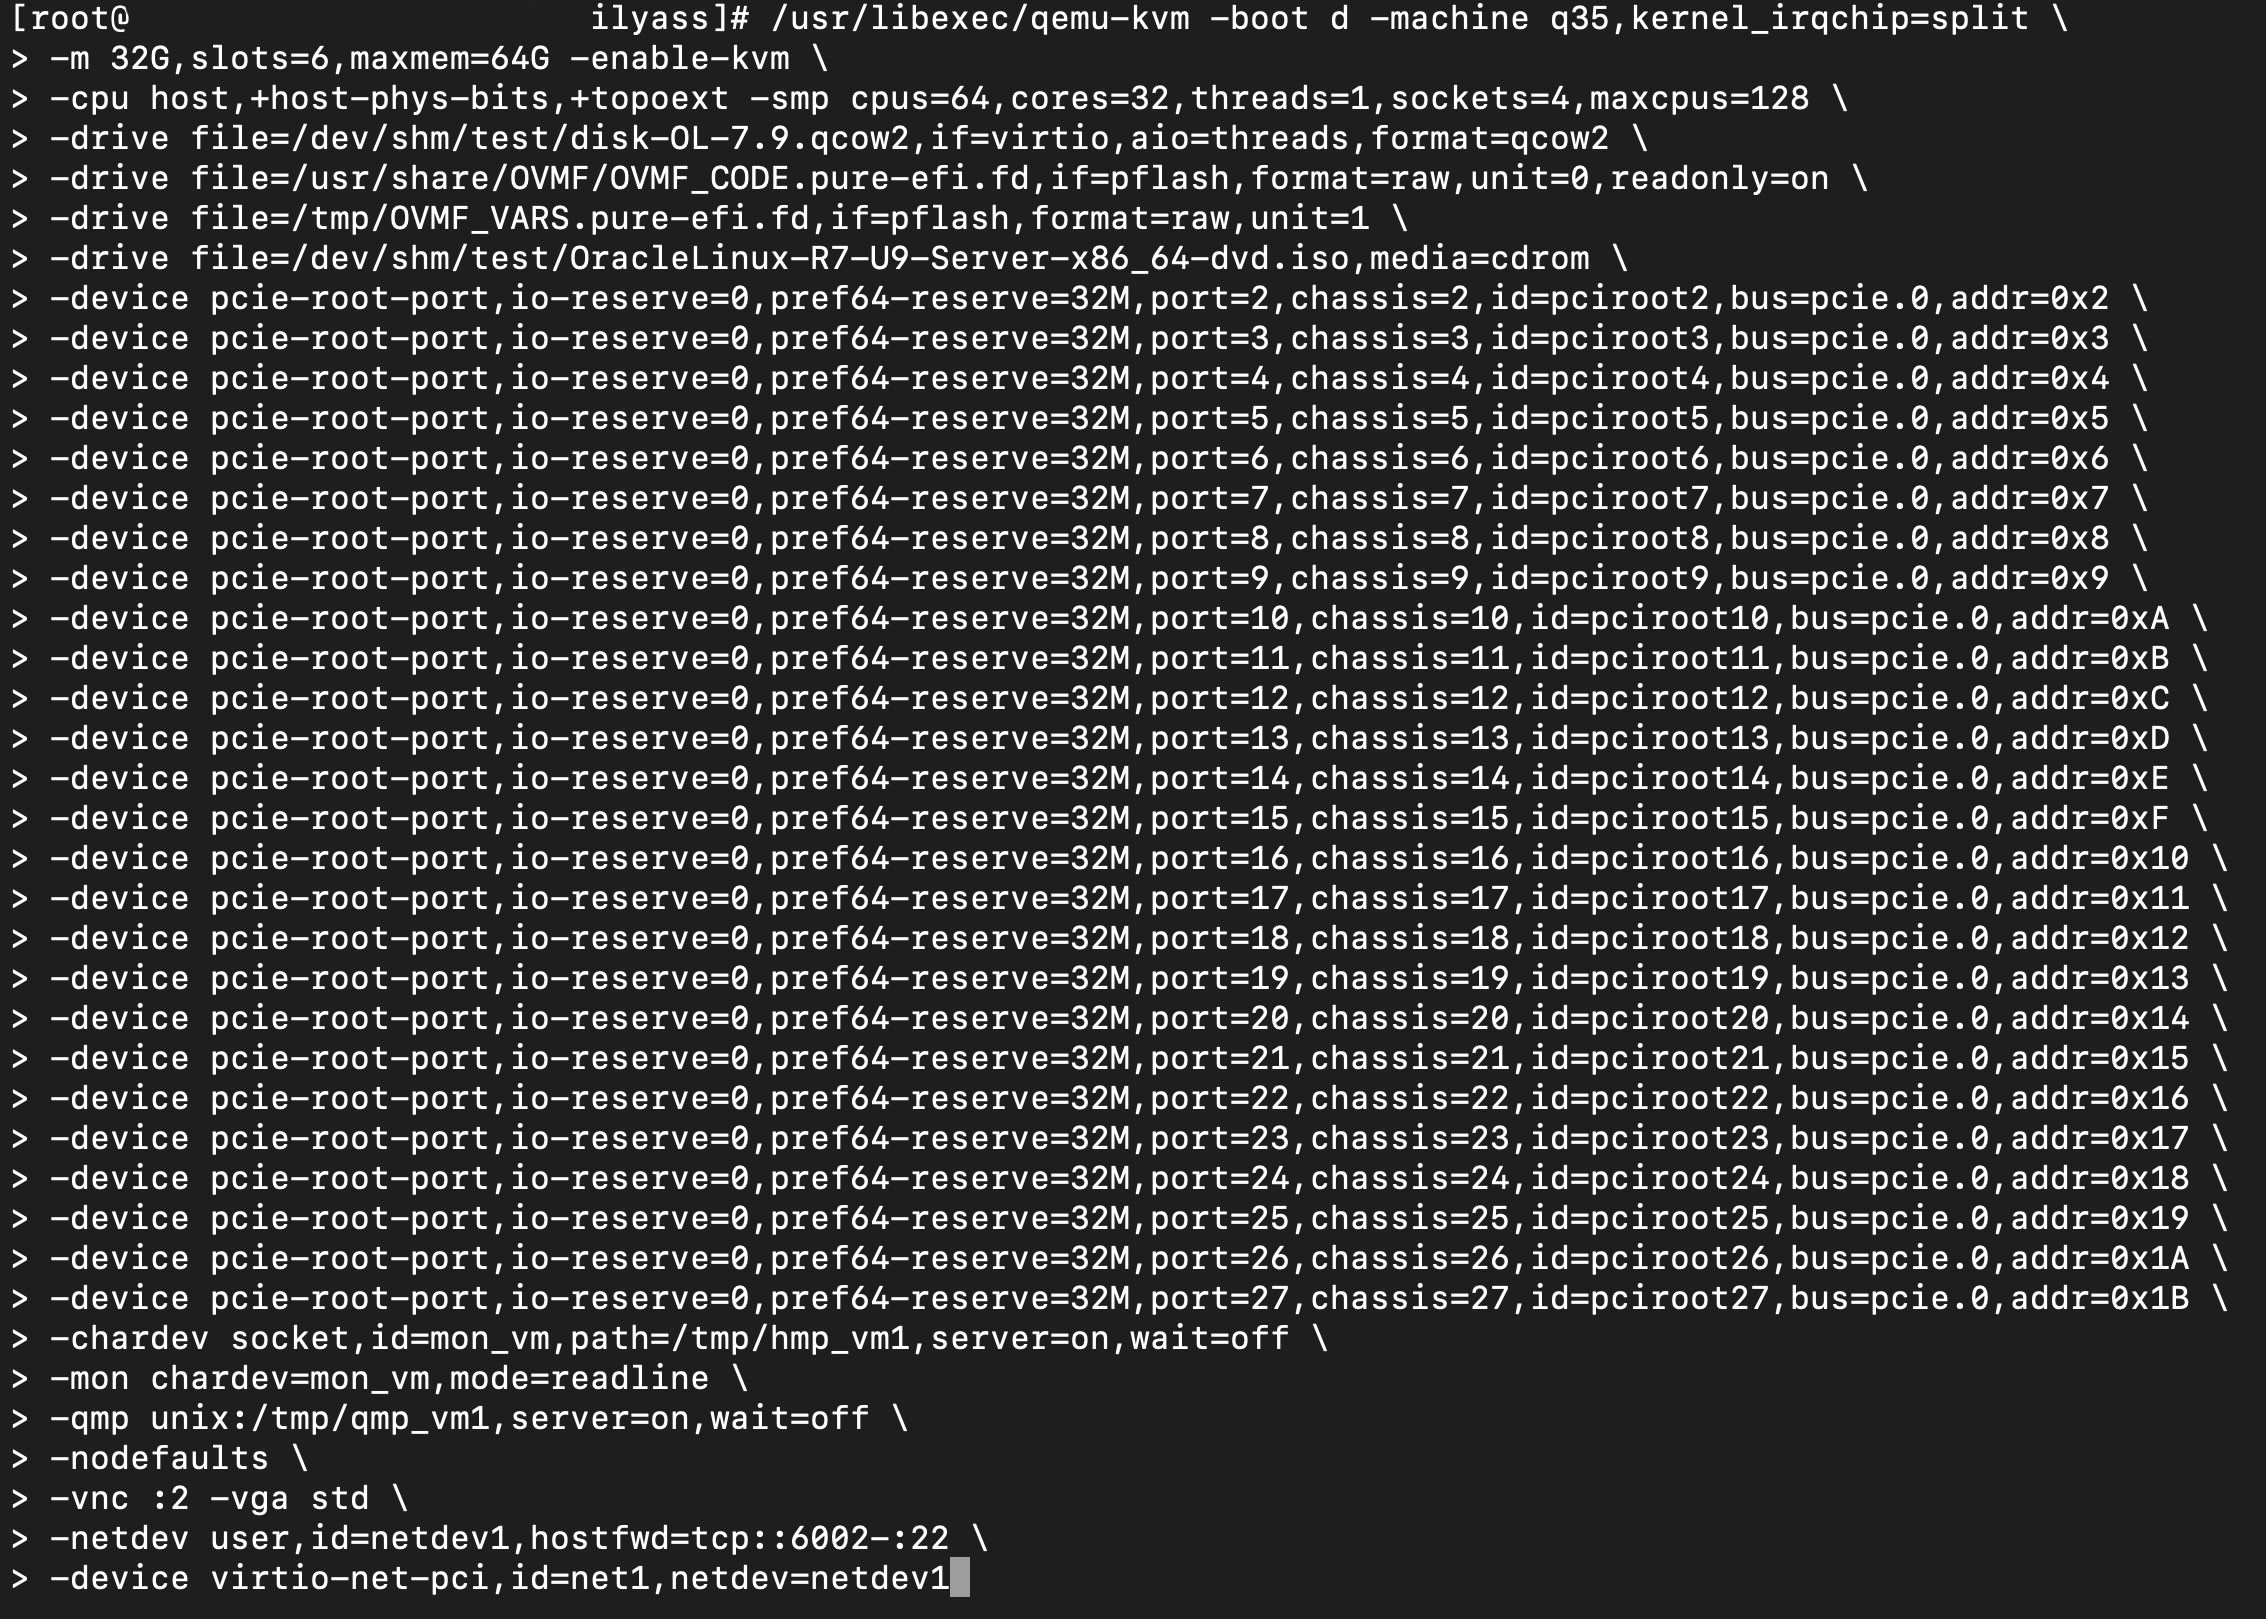
\includegraphics[width=\textwidth]{Images/Launching Guest 2.png}
    \captionof{figure}{QEMU Command for Launching the Guest}
    \label{fig:casa}
\end{center}

%% Test Execution and Performance Evaluation 
\subsection{Test Execution and Performance Evaluation}
Following the setup, a series of tests were conducted to evaluate the stability and performance of the virtual environment. These tests focused on the VM's lifecycle operations, the dynamic management of virtual network interfaces, the kdump check and dynamic add and removal of virtual CPUs.

%% Lifecycle Test 
\subsubsection[Lifecycle Test]{Lifecycle Test}

The lifecycle test assessed the VM’s ability to manage various operational states, including reboot, stop/continue, suspend, and shutdown. Each state transition was tested to ensure smooth operation and stability:
\noindent

\begin{itemize}
    \item \textbf{Reboot Test: }
          \begin{center}
              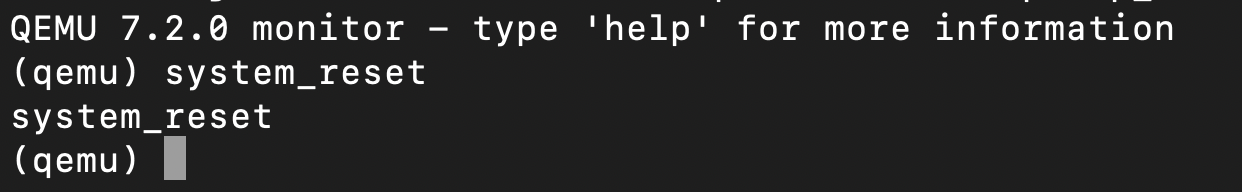
\includegraphics[width=\linewidth]{Images/Rebooting the Guest.png}
              \captionof{figure}{Execution of Reboot Command on the Guest}
              \label{fig:reboot}
          \end{center}
          \noindent
          \mynewline
    \item \textbf{Stop/Continue Test:}
          \begin{center}
              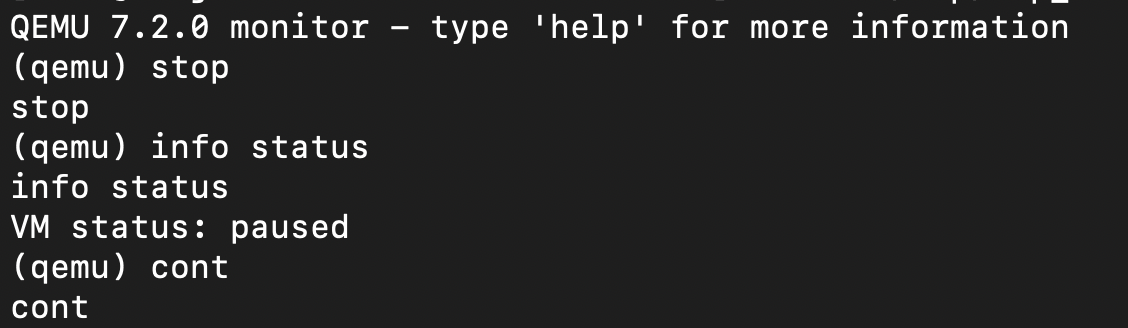
\includegraphics[width=\linewidth]{Images/Stop-Cont 2.png}
              \captionof{figure}{Stop and Continue Commands Executed on the Guest}
              \label{fig:areboot}
          \end{center}

    \item \textbf{Suspend Test:}
          \begin{center}
              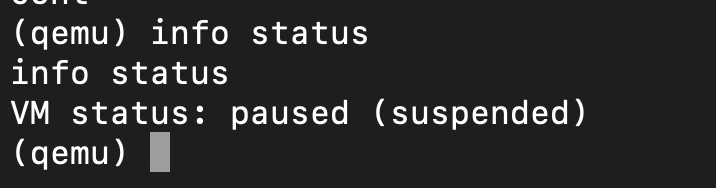
\includegraphics[width=\linewidth]{Images/Suspend Guest 2.png}
              \captionof{figure}{Guest Suspension via Systemctl Command}
              \label{fig:areboot}
          \end{center}

    \item \textbf{Shutdown Test:}
          \begin{center}
              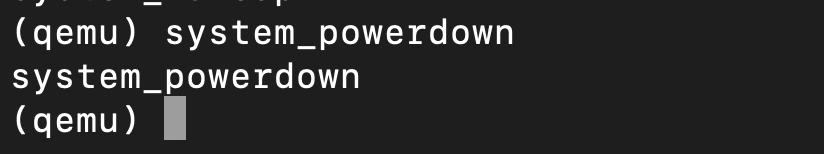
\includegraphics[width=\linewidth]{Images/System-powerdown.png}
              \captionof{figure}{Executing Shutdown Test on the Guest}
              \label{fig:areboot}
          \end{center}
\end{itemize}

All lifecycle tests were executed successfully, demonstrating the VM's capability to handle various operational states without issues. Each command transitioned smoothly, confirming the stability and reliability of the virtual environment.

%% Some VNIC Hotplug/Unplug 
\subsubsection[Some VNIC Hotplug/Unplug]{Some VNIC Hotplug/Unplug}

The hotplug and unplug test of VNICs was conducted to simulate high-density networking scenarios. This involved dynamically adding and removing multiple VNICs from the VM.\mynewline

Before initiating the test, we established a baseline by listing the existing network interfaces using the ip a command. The previous script, VNIC\_Hotplug.sh, was used to automate the addition of VNICs.\mynewline

The addition of VNICs was verified through system logs and updated network configurations. Following the hotplug, we confirmed that all interfaces were successfully added and configured:

\begin{center}
    \centering
    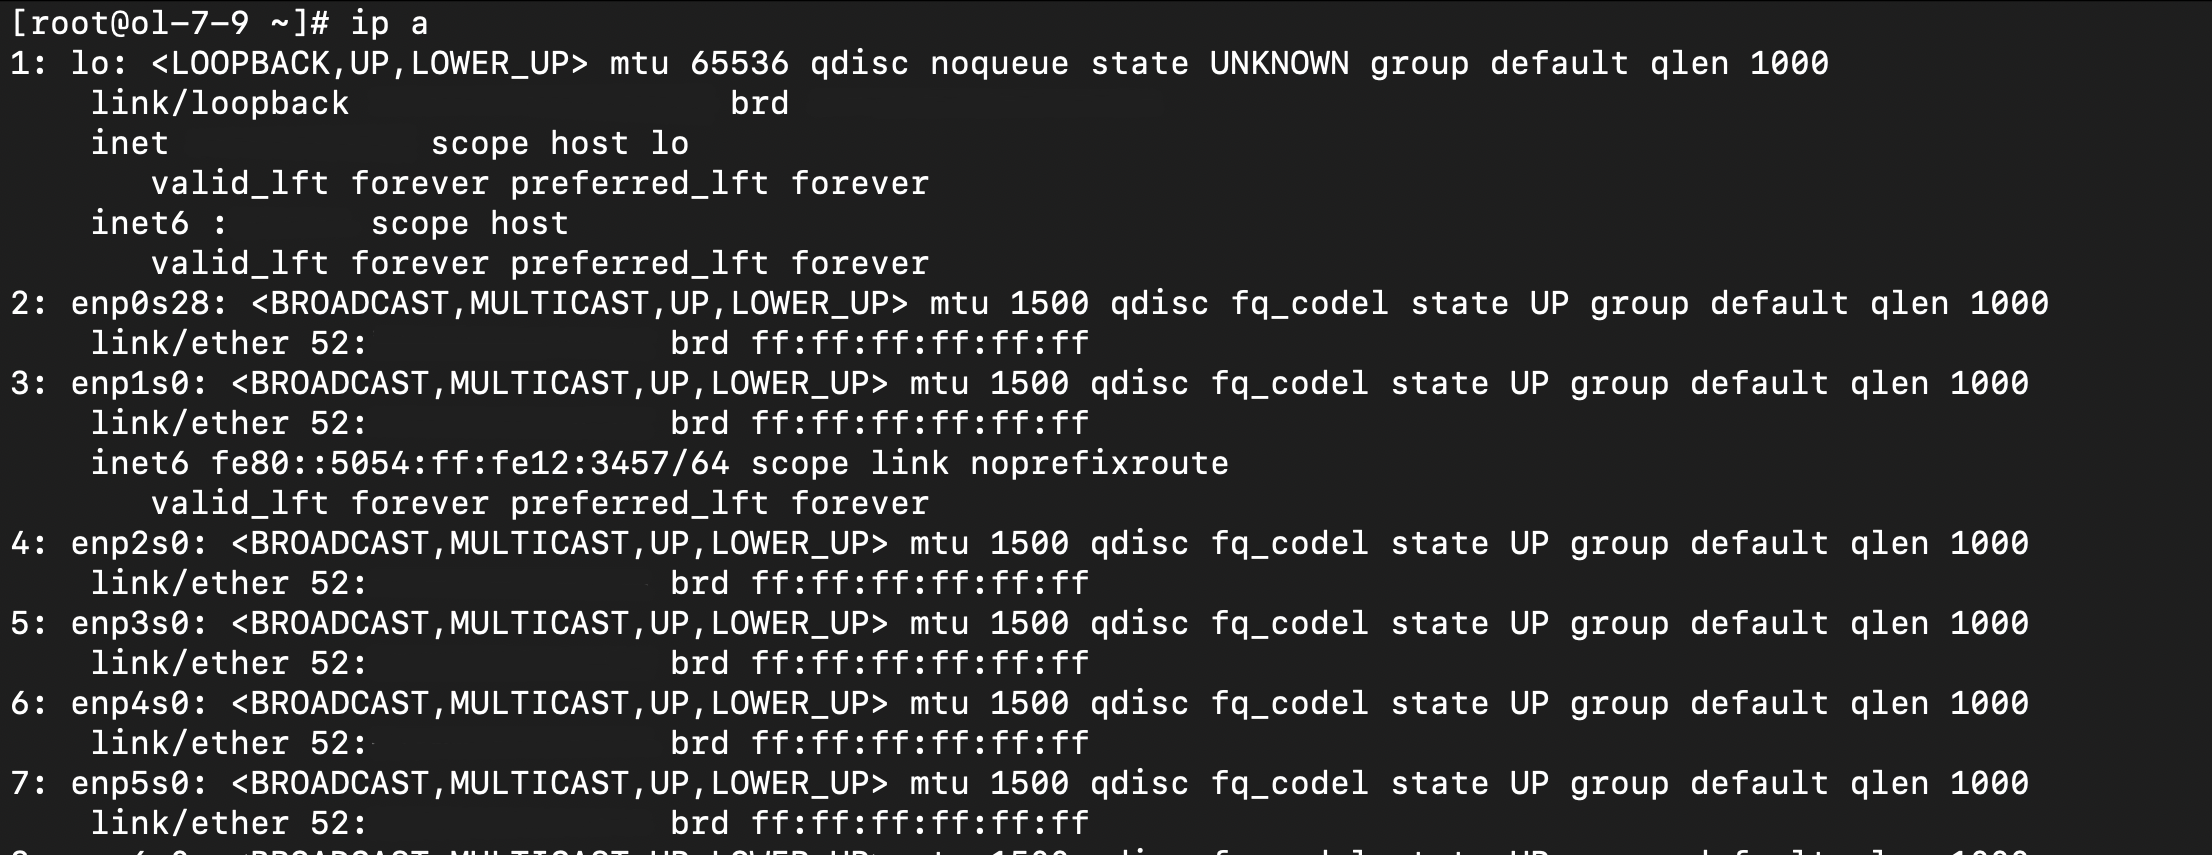
\includegraphics[width=\textwidth]{Images/ip a after VNIC Hotplug 2.png}
    \captionof{figure}{Post-Hotplug Network Interface List in the Guest}
    \label{fig:casa}
\end{center}

For the unplug process, the script VNIC\_Unplug.sh removed each VNIC systematically. The removal was verified by checking the updated network interface list.

%% VFIO-VNIC Hotplug/Unplug 
\subsubsection[Some VFIO-VNIC Hotplug/Unplug]{Some VFIO-VNIC Hotplug/Unplug}

In this test, some VFIO VNICs were managed on the host system. The hotplug process was verified through the QEMU monitor commands (VFIO\_VNIC\_Hotplug.sh) and confirmed by updated network interface lists in the guest VM:

\begin{center}
    \centering
    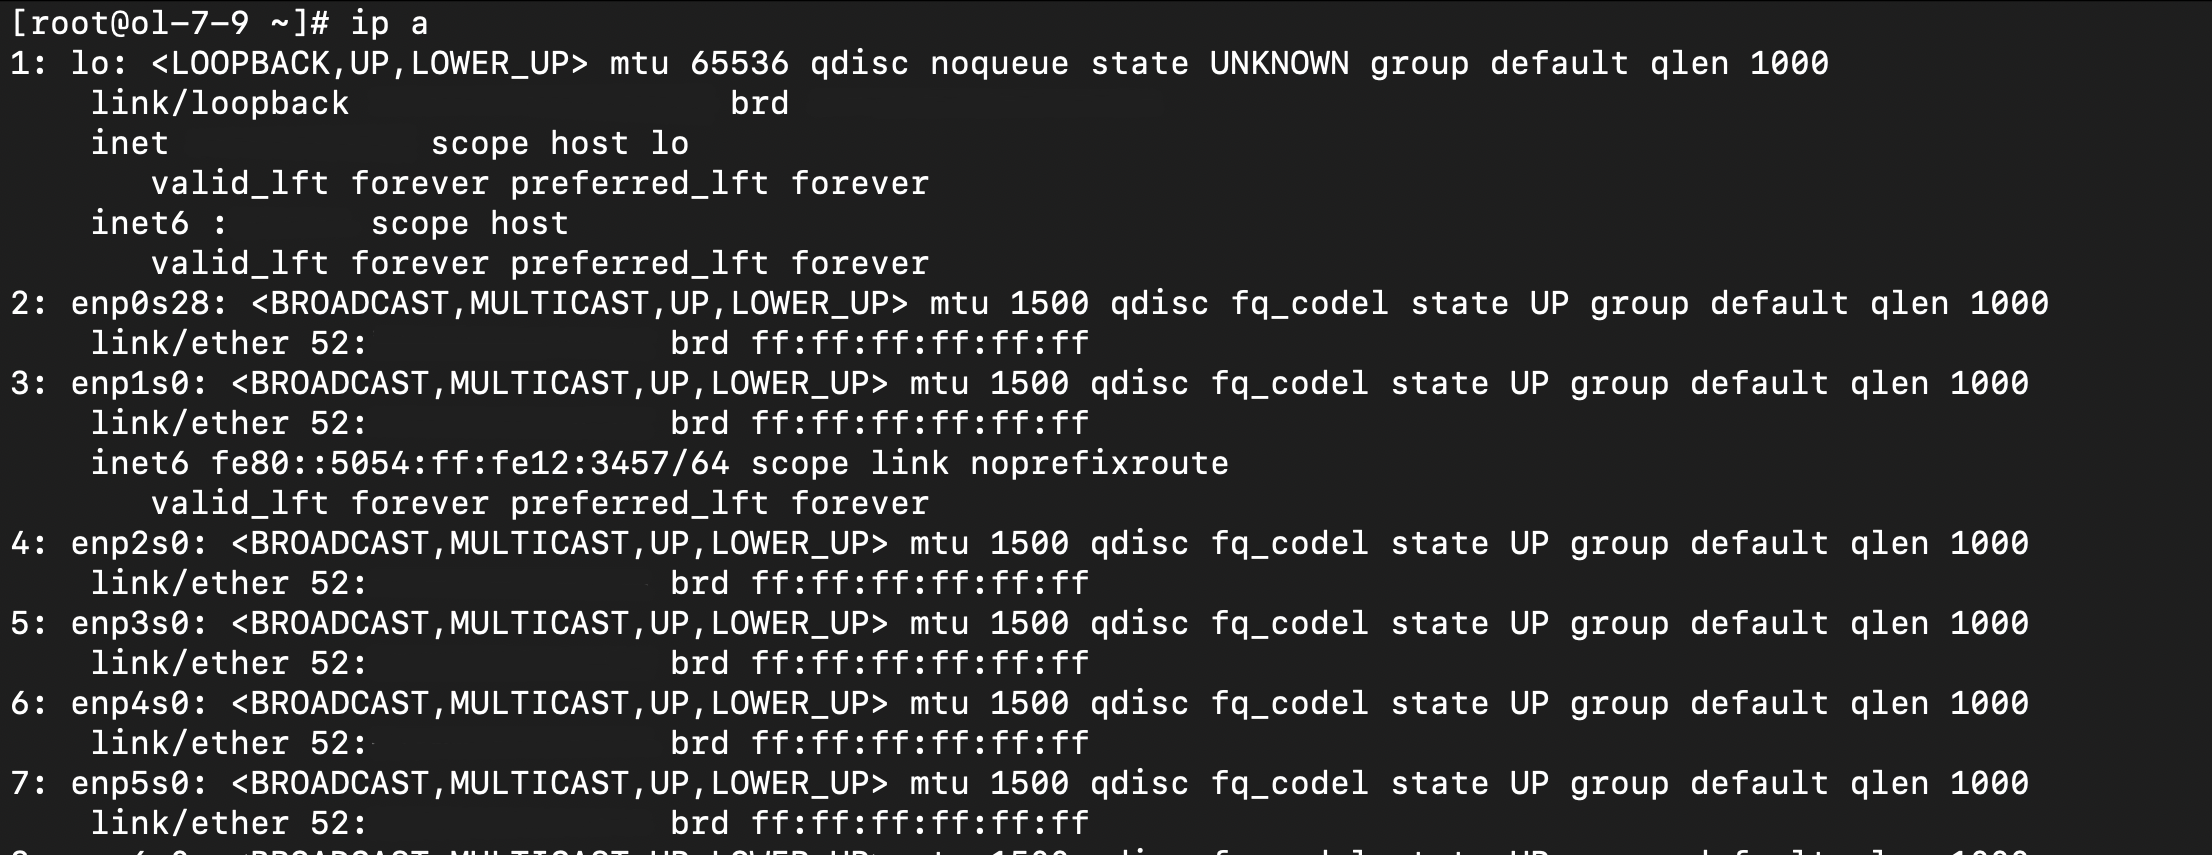
\includegraphics[width=\textwidth]{Images/ip a after VNIC Hotplug 2.png}
    \captionof{figure}{Network Interface List After VFIO VNIC Hotplug}
    \label{fig}
\end{center}

The unplug process was similarly executed, and the network interface list was checked to confirm successful removal of VFIO VNICs.

%% 3 vDisk Hotplug/Unplug 
\subsubsection[VDisks Hotplug/Unplug]{VDisks Hotplug/Unplug}
The vDisk images were prepared on the host and used for the hotplug/unplug test. The disks were created and added to the VM using QEMU commands are located on \texttt{/home/opc} path, with verification through the lsblk command before and after the hotplug:

\begin{center}
    \centering
    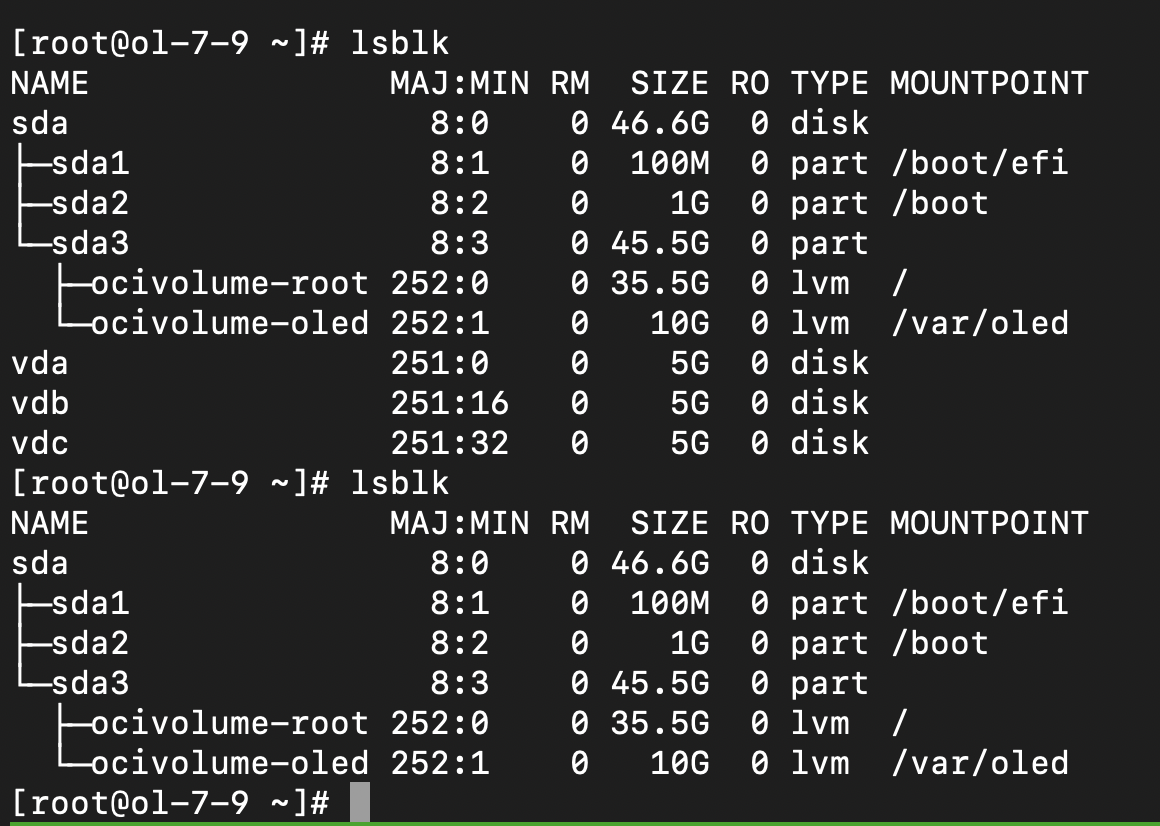
\includegraphics[width=\textwidth]{Images/lsblk after hotplug and after ungplug.png}
    \captionof{figure}{Updated Block Device List Post-Hotplug and Unplug}
    \label{fig}
\end{center}

%% Kdump Check
\subsubsection[Kdump Check]{Kdump Check}
To verify the Kdump functionality, we configured the system to capture crash dumps in the event of kernel failures:

\begin{center}
    \centering
    \includegraphics[width=\textwidth]{Images/Kdump Test 2.png}
    \captionof{figure}{Initiating Kdump Process}
    \label{fig}
\end{center}

\begin{center}
    \centering
    \includegraphics[width=\textwidth]{Images/Log Folder Founded.png}
    \captionof{figure}{Crash Dump Directory Verification}
    \label{fig}
\end{center}

The Kdump functionality was further validated by analyzing the crash dump files, confirming that the crash data was accurately captured and processed.

%% VCPUs Hotplug/Unplug
\subsubsection[VCPUs Hotplug/Unplug]{VCPUs Hotplug/Unplug}
The vCPU hotplug test involved dynamically adding and removing virtual CPUs from the guest VM to evaluate its capability to handle changes in CPU resources.\mynewline

Initially, the VM was configured with a certain number of CPUs. To perform the hotplug test, we used the following QEMU monitor commands to add three additional vCPUs:

\begin{center}
    \centering
    \includegraphics[width=\textwidth]{Images/Hotplug cpu.png}
    \captionof{figure}{Executing vCPU Hotplug Process}
    \label{fig}
\end{center}

Before the hotplug operation and after it, the VM’s CPU configuration was as follows:

\begin{center}
    \centering
    \includegraphics[width=\textwidth]{Images/lscpu before hotplug.png}
    \captionof{figure}{CPU Configuration Before Hotplug}
    \label{fig}
\end{center}

\begin{center}
    \centering
    \includegraphics[width=\textwidth]{Images/lscpu after hotplug.png}
    \captionof{figure}{CPU Configuration After Hotplug}
    \label{fig}
\end{center}

Following the vCPU addition, we tested the vCPU unplug process using similar QEMU monitor commands to remove the added CPUs. The CPU configuration reverted to its original state, this confirmed the successful dynamic adjustment of vCPUs in the VM.

%% Overview of Testing Outcomes
\subsubsection[Overview of Testing Outcomes]{Overview of Testing Outcomes}
The testing conducted for QEMU on AMD host with OL8 + UEK7U2 and OL 7.9 + UEK6U3 guest revealed several key insights:

\begin{itemize}
    \item \textbf{Lifecycle Operations:} The guest VM managed various operational states, including reboot, stop/continue, suspend, and shutdown, effectively and without issues. Each state transition was smooth, demonstrating robust lifecycle management capabilities;
    \item \textbf{Hotplug/Unplug of VNICs:} The system successfully handled the dynamic addition and removal of virtual network interfaces (VNICs), with all interfaces being correctly recognized and configured. This indicates strong support for high-density networking scenarios;
    \item \textbf{VFIO-VNIC Hotplug/Unplug:} The VFIO VNICs were managed successfully, with the system effectively adding and removing the VFIO VNICs. The network interface list was updated as expected, showing the VM’s capability to handle VFIO network interfaces;
    \item \textbf{VDisk Hotplug/Unplug:} The test demonstrated that the VM could efficiently attach and detach virtual disks, with the system accurately reflecting the changes in disk availability and configuration;
    \item \textbf{Kdump Functionality:} The Kdump test validated that the system could capture and store crash dumps correctly, with dump files being successfully created and analyzed following a kernel panic;
    \item \textbf{VCPU Hotplug/Unplug:} The dynamic addition and removal of vCPUs were executed successfully, with the VM reflecting changes in CPU configuration as expected. This tested the VM's capability to handle varying CPU resources effectively.
\end{itemize}

Overall, the tests confirmed that the virtual environment operated within the expected parameters, demonstrating stability, reliability, and proper functionality of key virtualization features.

%% OL8 virt:kvm_utils3 Release 10 libvirt 9.0.0-6/Qemu 7.2.0-15 non OCI Linux Guest (OL 8.10) Manual Sanity Test on A1-2c libvirt initiated
\section{Test on OL8 Host with and ARM CPU, Libvirt, QEMU and Latest kernel version UEK7U2}

%% Host System and Guest VM Configuration 
\subsection{Host System and Guest VM Configuration}

For this testing phase, an ARM-based OCI instance was utilized, running Oracle Linux Server 8. The host system was equipped with the latest UEK7U2 kernel, and the configuration process commenced with the installation of QEMU and Libvirt. Ensuring the correct installation and environment setup was paramount to the success of the tests.\mynewline

The initial verification procedures involved confirming the host system's details via the \texttt{hostnamectl} command, followed by a thorough check of all QEMU and Libvirt components:

\begin{center}
    \centering
    \includegraphics[width=\textwidth]{Images/Host System Config 3.png}
    \captionof{figure}{Verification of Host System Configuration}
    \label{fig:casa}
\end{center}

With the host system confirmed to be in optimal condition, the next step was deploying the guest VM, which ran Oracle Linux 8.10 with UEK7U2. The VM was launched using a Libvirt script, ensuring proper initialization for the upcoming testing phase:

\begin{center}
    \centering
    \includegraphics[width=\textwidth]{Images/Launching Guest 3.png}
    \captionof{figure}{Deployment Script for the Guest via Libvirt}
    \label{fig:casa}
\end{center}

%% Test Execution and Performance Evaluation 
\subsection{Test Execution and Performance Evaluation}
Following the setup, various tests were executed to evaluate the stability and performance of the virtual environment. These tests focused on the VM's lifecycle management, the dynamic handling of VNICs, and kdump testing, and the booting of large VMs.

%% Lifecycle Test 
\subsubsection[Lifecycle Test]{Lifecycle Test}

The lifecycle test was designed to assess the VM’s capability to handle different operational states, including start, reboot, suspend, resume, reset and shutdown. Each transition was meticulously tested to ensure seamless operation and system stability:

\begin{itemize}
    \item \textbf{Start Test:}
          \begin{center}
              \includegraphics[width=\linewidth]{Images/Start using libvirt.png}
              \captionof{figure}{Execution of Start Command on the Guest}
              \label{fig:reboot}
          \end{center}

    \item \textbf{Reboot Test:}
          \begin{center}
              \includegraphics[width=\linewidth]{Images/Reboot using libvirt.png}
              \captionof{figure}{Execution of Reboot Command on the Guest}
              \label{fig:reboot}
          \end{center}

    \item \textbf{Suspend Test:}
          \begin{center}
              \includegraphics[width=\linewidth]{Images/Suspend using libvirt.png}
              \captionof{figure}{Suspension of the Guest Using Libvirt}
              \label{fig:areboot}
          \end{center}

    \item \textbf{Resume Test:}
          \begin{center}
              \includegraphics[width=\linewidth]{Images/Resume using libvirt.png}
              \captionof{figure}{Resuming the Guest After Suspension}
              \label{fig:areboot}
          \end{center}

    \item \textbf{Reset Test:}
          \begin{center}
              \includegraphics[width=\linewidth]{Images/Reset Using libvirt.png}
              \captionof{figure}{Reset Command Execution on the Guest}
              \label{fig:areboot}
          \end{center}

    \item \textbf{Shutdown Test:}
          \begin{center}
              \includegraphics[width=\linewidth]{Images/Shutdown using Libvirt.png}
              \captionof{figure}{Guest Shutdown Initiated via Libvirt}
              \label{fig:areboot}
          \end{center}
\end{itemize}

The lifecycle tests were successfully completed, with each command executing flawlessly, confirming the VM’s robust lifecycle management capabilities.

%% Some VNIC Hotplug/Unplug 
\subsubsection[Some VNIC Hotplug/Unplug]{Some VNIC Hotplug/Unplug}

A script was employed to automate the hotplugging of some VNICs using Libvirt:

\begin{center}
    \centering
    \includegraphics[width=\textwidth]{Images/Script hotplug VNIC Libvirt.png}
    \captionof{figure}{Libvirt Script for VNIC Hotplug}
    \label{fig:casa}
\end{center}

The successful addition of the VNICs was verified by examining the system logs and updated network configurations. Post-hotplugging, all interfaces were confirmed to be properly recognized and configured:

\begin{center}
    \centering
    \includegraphics[width=\textwidth]{Images/ip a after hotplug VNIC Libvirt.png}
    \captionof{figure}{Post-Hotplug Verification of Network Interfaces}
    \label{fig:casa}
\end{center}

For the unplugging process, a script was executed to systematically remove each VNIC. The removal was validated by verifying the updated network interface list which contains just two.

%% VFIO-VNIC Hotplug/Unplug 
\subsubsection[Some VFIO-VNIC Hotplug/Unplug]{Some VFIO-VNIC Hotplug/Unplug}

This test focused on managing VFIO VNICs on the host system. The hotplugging process was carried out using Libvirt scripts, with the following steps verified:

\begin{center}
    \centering
    \includegraphics[width=\textwidth]{Images/Populate VFIO libvirt.png}
    \captionof{figure}{Populating VFIO Files via Script}
    \label{fig}
\end{center}

\begin{center}
    \centering
    \includegraphics[width=\textwidth]{Images/VFIO VNIC Hotplug Libvirt.png}
    \captionof{figure}{Hotplugging VFIO VNIC Using Libvirt}
    \label{fig}
\end{center}

\begin{center}
    \centering
    \includegraphics[width=\textwidth]{Images/ip a after hotplug vfio libvirt.png}
    \captionof{figure}{Updated Network Interface List After VFIO Hotplug}
    \label{fig}
\end{center}

The hotplugging operation was successfully completed, with the network interface list reflecting the newly added VFIO VNICs on the guest VM. The unplugging process was executed similarly, and the network interface list confirmed the successful removal of the VFIO VNICs.

%% VDisk Hotplug/Unplug 
\subsubsection[VDisks Hotplug/Unplug]{VDisks Hotplug/Unplug}

Some vDisks were created on the host in the \texttt{/dev/shm/ilyass/images/} directory for the hotplug/unplug tests. The disks were added to the VM using Libvirt commands, and the operation was verified using the \texttt{lsblk} command before and after the hotplug:

\begin{center}
    \centering
    \includegraphics[width=\textwidth]{Images/lsblk after hotplug and after ungplug.png}
    \captionof{figure}{Verifying Block Device List After Hotplug and Unplug}
    \label{fig}
\end{center}

%% Kdump Check
\subsubsection[Kdump Check]{Kdump Check}

To test Kdump functionality, the system was configured to capture crash dumps during kernel failures:

\begin{center}
    \centering
    \includegraphics[width=\textwidth]{Images/kdump test 3.png}
    \captionof{figure}{Executing Kdump Process on the Guest}
    \label{fig}
\end{center}

\begin{center}
    \centering
    \includegraphics[width=\textwidth]{Images/Kdumpt Result folder.png}
    \captionof{figure}{Crash Dump Files Stored in Kdump Directory}
    \label{fig}
\end{center}

The Kdump functionality was confirmed by analyzing the captured crash dump files, which verified that the crash data was accurately recorded and processed.

%% Big VM 500G-1T Boot Test 
\subsubsection[Big VM 500G-1T Boot Test]{Big VM 500G-1T Boot Test}

A VM with a configuration of 500G GB RAM and then 1000G GB RAM was deployed to test the environment's capability to handle large VM instances. The VM was successfully booted, and the expected resource allocation was verified via the \texttt{lsmem} command:

\begin{center}
    \centering
    \includegraphics[width=\textwidth]{Images/Large VM Test 500G.png}
    \captionof{figure}{Resource Allocation Verification in Large VM (500G RAM)}
    \label{fig}
\end{center}

\begin{center}
    \centering
    \includegraphics[width=\textwidth]{Images/Large VM Test 1T.png}
    \captionof{figure}{Resource Allocation Verification in Large VM (1T RAM)}
    \label{fig}
\end{center}

The successful boot of the large VM confirmed that the environment was capable of handling resource-intensive virtual machines without issues.

\subsubsection[Overview of Testing Outcomes]{Overview of Testing Outcomes}

In this testing phase, we evaluated the performance and stability of the virtual environment on an ARM-based OCI instance running Oracle Linux Server 8 with UEK7U2. The key aspects of this testing involved lifecycle management, virtual network interface handling, virtual disk operations, kdump functionality, and the booting of large VMs. The outcomes of these tests are summarized below:

\begin{itemize}
    \item \textbf{Lifecycle Operations:} The VM demonstrated robust lifecycle management by successfully executing start, reboot, suspend, resume, reset, and shutdown operations. Each state transition was smooth, indicating that the environment can handle various operational states without disruptions;

    \item \textbf{Hotplug/Unplug of VNICs:} The VM efficiently managed the dynamic addition and removal of virtual network interfaces using Libvirt. All network interfaces were correctly recognized and configured, demonstrating the system's ability to support high-density networking requirements;

    \item \textbf{Hotplug/Unplug of VFIO VNICs:} The test confirmed that the VM could effectively manage VFIO VNICs. The successful hotplugging and unplugging operations reflected the environment's capability to handle VFIO-based network interfaces, which are critical for direct device access in virtualized environments;

    \item \textbf{VDisks Hotplug/Unplug:} The VM successfully attached and detached the virtual disks. The system accurately reflected the changes in disk availability, confirming the environment’s ability to manage dynamic storage configurations effectively;

    \item \textbf{Kdump Functionality:} The Kdump test validated the system’s ability to capture and store crash dumps. The dump files were correctly generated and analyzed, demonstrating the reliability of the crash recovery process;

    \item \textbf{Large VM Boot Test (500G-1T RAM):} The successful boot of a VM with 500G and then 1000G RAM confirmed the environment's capacity to handle large, resource-intensive virtual machines. The test validated the system's scalability and its ability to allocate significant resources without issues.
\end{itemize}

Overall, the testing confirmed that the virtual environment is stable, reliable, and capable of handling a wide range of demanding virtualization scenarios. The system operated within expected parameters, and all tested features performed as anticipated.

\section{Conclusion}
In conclusion, this chapter detailed the implementation and testing of QEMU with various configurations. It highlighted the technical choices made, the execution of tests, and the validation results, demonstrating the system’s functionality and readiness for practical use.